% Credits are indicated where needed. The general idea is based on a template by Vel (vel@LaTeXTemplates.com) and Frits Wenneker.

\documentclass[11pt, a4paper]{article} % General settings in the beginning (defines the document class of your paper)
% 11pt = is the font size
% A4 is the paper size
% “article” is your document class
\usepackage{color,soul}
\usepackage{url}
\usepackage{graphicx}
%----------------------------------------------------------------------------------------
%	Packages
%----------------------------------------------------------------------------------------

% Necessary
\usepackage[german,english]{babel} % English and German language 
\usepackage{booktabs} % Horizontal rules in tables 
% For generating tables, use “LaTeX” online generator (https://www.tablesgenerator.com)
\usepackage{comment} % Necessary to comment several paragraphs at once
\usepackage[utf8]{inputenc} % Required for international characters
\usepackage[T1]{fontenc} % Required for output font encoding for international characters

% Might be helpful
\usepackage{amsmath,amsfonts,amsthm} % Math packages which might be useful for equations
\usepackage{tikz} % For tikz figures (to draw arrow diagrams, see a guide how to use them)
\usepackage{tikz-cd}
\usetikzlibrary{positioning,arrows} % Adding libraries for arrows
\usetikzlibrary{decorations.pathreplacing} % Adding libraries for decorations and paths
\usepackage{tikzsymbols} % For amazing symbols ;) https://mirror.hmc.edu/ctan/graphics/pgf/contrib/tikzsymbols/tikzsymbols.pdf 
\usepackage{blindtext} % To add some blind text in your paper


%---------------------------------------------------------------------------------
% Additional settings
%---------------------------------------------------------------------------------

%---------------------------------------------------------------------------------
% Define your margins
\usepackage{geometry} % Necessary package for defining margins

\geometry{
	top=2cm, % Defines top margin
	bottom=2cm, % Defines bottom margin
	left=2.2cm, % Defines left margin
	right=2.2cm, % Defines right margin
	includehead, % Includes space for a header
	%includefoot, % Includes space for a footer
	%showframe, % Uncomment if you want to show how it looks on the page 
}

\setlength{\parindent}{15pt} % Adjust to set you indent globally 

%---------------------------------------------------------------------------------
% Define your spacing
\usepackage{setspace} % Required for spacing
% Two options:
\linespread{1.5}
%\onehalfspacing % one-half-spacing linespread

%----------------------------------------------------------------------------------------
% Define your fonts
\usepackage[T1]{fontenc} % Output font encoding for international characters
\usepackage[utf8]{inputenc} % Required for inputting international characters

\usepackage{XCharter} % Use the XCharter font


%---------------------------------------------------------------------------------
% Define your headers and footers

\usepackage{fancyhdr} % Package is needed to define header and footer
\pagestyle{fancy} % Allows you to customize the headers and footers

%\renewcommand{\sectionmark}[1]{\markboth{#1}{}} % Removes the section number from the header when \leftmark is used

% Headers
\lhead{} % Define left header
\chead{\textit{}} % Define center header - e.g. add your paper title
\rhead{} % Define right header

% Footers
\lfoot{} % Define left footer
\cfoot{\footnotesize \thepage} % Define center footer
\rfoot{ } % Define right footer

%---------------------------------------------------------------------------------
%	Add information on bibliography
\usepackage{natbib} % Use natbib for citing
\usepackage{har2nat} % Allows to use harvard package with natbib https://mirror.reismil.ch/CTAN/macros/latex/contrib/har2nat/har2nat.pdf

% For citing with natbib, you may want to use this reference sheet: 
% http://merkel.texture.rocks/Latex/natbib.php

%---------------------------------------------------------------------------------
% Add field for signature (Reference: https://tex.stackexchange.com/questions/35942/how-to-create-a-signature-date-page)
\newcommand{\signature}[2][5cm]{%
  \begin{tabular}{@{}p{#1}@{}}
    #2 \\[2\normalbaselineskip] \hrule \\[0pt]
    {\small \textit{Signature}} \\[2\normalbaselineskip] \hrule \\[0pt]
    {\small \textit{Place, Date}}
  \end{tabular}
} % Loads required packages from the separate file 

%---------------------------------------------------------------------------------
%	General information
%---------------------------------------------------------------------------------
\title{Omnichain Web: A Comprehensive Overview} % Adds your title
\author{
Dojima Foundation % Add your first and last name
\\www.dojima.foundation
    %\thanks{} % Adds a footnote to your title
    %\institution{YOUR INSTITUTION} % Adds your institution
  }

\date{\small Preliminary Draft, January 11, 2025} % Adds the current date to your “cover” page; leave empty if you do not want to add a date


%---------------------------------------------------------------------------------
%	Define what’s in your document
%---------------------------------------------------------------------------------
\AtBeginDocument{\addtocontents{toc}{\protect\thispagestyle{empty}}}
\begin{document}

% If you want a cover page, uncomment "\input{content/0A-coverpage}" and comment "\maketitle" as well as "\input{content/0B-disclaimer}"

\maketitle % Print your title, author name and date; comment if you want a cover page 
%\input{content/0A-coverpage} % Adds a cover page; uncomment if you want a cover page
%\input{content/0B-disclaimer} % Gives you the word count; comment if you want a cover page 
%---------------------------------------------------------------------------------
% Abstract
%---------------------------------------------------------------------------------
\thispagestyle{empty}
\begin{abstract}
\text{ }\\
The rapid evolution of blockchain technology is being hindered by the fragmentation of blockchain ecosystems, with thousands of independent chains lacking interoperability. Cross-chain communication has emerged as a key challenge, with significant barriers originating from various protocols, consensus mechanisms, and data structures. Omnichain Web offers a groundbreaking solution to this problem by providing a unified framework that enables seamless interaction across multiple blockchains with different architecture and languages, including Layer 1 (L1), Layer 2 (L2), and any emerging ecosystems. By abstracting the complexities of cross-chain interoperability, Omnichain Web ensures a frictionless and secure environment for decentralized applications (dApps), eliminating fragmentation and dependency bottlenecks that have plagued traditional solutions. 

The Omnichain Web ecosystem consists of four core components: the Builder Marketplace, Omni Sequencer, Prover Network, and Ragno Network, which together facilitate secure, scalable, and future-proof cross-chain operations. This holistic approach empowers developers and businesses to innovate without worrying about the limitations of individual blockchain ecosystems. As the Web3 ecosystem continues to expand, Omnichain Web's omnichain capabilities set the stage for a seamless connection between Web2 and Web3, offering decentralized services that are both secure and scalable. This paper explores the future of cross-chain interoperability, the challenges of integrating Web2 entities into Web3, and the transformative potential of Omnichain Web in shaping the decentralized future.


\end{abstract} % Adds your abstract
%---------------------------------------------------------------------------------
% Table of content
%---------------------------------------------------------------------------------

\newpage % Generates page break

% Table of content
\thispagestyle{empty} % Suppresses page numbers
\small
\tableofcontents % Adds table of content
\normalsize
\newpage % Generates page break

% List of figures
%\thispagestyle{empty} % Suppresses page numbers
%\listoffigures % Adds list of figures; uncomment if required
%\newpage % Generates page break; uncomment if required

% List of tables
%\thispagestyle{empty} % Suppresses page numbers
%\listoftables % Adds list of tables; uncomment if required
%\newpage % Generates page break; uncomment if required
 % Adds a table of content; uncomment if required


%----------------------------------------------------------------------------------------
% Introduction
%----------------------------------------------------------------------------------------
\setcounter{page}{1} % Sets counter of page to 1

\section{Introduction} % Add a section title

\subsection{Importance of Cross-Chain Interoperability in Blockchain} 

In the early days of the Internet, on-line systems were fragmented. Different networks operated in isolation, each with its proprietary protocols, making it difficult for users to access and exchange information seamlessly. This fragmented approach stifled innovation and limited the potential of the Internet. The advent of the World Wide Web, with its standard protocols like HTTP and TCP/IP, transformed this landscape by enabling universal connectivity~\cite{www}. It created a unified, interoperable platform that revolutionized global communication, commerce, and collaboration. Similarly, blockchain technology today faces a comparable challenge: Thousands of independent blockchains operate as siloed ecosystems, each with its own protocols, standards, and functionality.

Cross-chain operability is the blockchain equivalent of the standardization brought about by the World Wide Web. By allowing different blockchain networks to communicate and interact seamlessly, it unlocks the full potential of decentralized technologies. Users can transfer assets, share data, and execute smart contracts across multiple chains without having to navigate the technical and logistical complexities of each. This interoperability fosters innovation by allowing developers to build decentralized applications (dApps) that leverage the strengths of multiple chains, be it scalability, security, or cost efficiency. It ensures that the blockchain ecosystem evolves as a cohesive, interconnected network, much like how the internet evolved into a global information superhighway.

As discussed in~\cite{crosschain}, one of the main challenges is the heterogeneity of blockchain platforms. Each blockchain operates with its own protocols, consensus mechanisms, and data structures, creating significant barriers to seamless interaction. This diversity leads to "disconnected value islands," where assets and data are confined within individual blockchains, limiting their utility and the broader potential of blockchain technology. Another critical issue is the security vulnerabilities inherent in cross-chain interactions. In~\cite{crosschain}, Harris, C. G. discusses various exploits and attacks that have targeted cross-chain bridges and interoperability protocols, underscoring the need for robust security measures. Ensuring the integrity and authenticity of transactions across different blockchains remains a formidable challenge. 

Despite these challenges, the article describes several opportunities to improve blockchain interoperability. The development and implementation of standardized protocols can facilitate more straightforward communication between disparate blockchains. By establishing common standards, interoperability solutions can be more easily adopted, promoting a more cohesive blockchain ecosystem~\cite{mao}. Furthermore, cross-chain technologies have high potential to foster innovation in decentralized applications (dApps). By enabling dApps to operate across multiple blockchains, developers can leverage the unique features and capabilities of different platforms, leading to more versatile and powerful applications. This cross-chain functionality can drive the next wave of growth and adoption in the blockchain space. 

\begin{figure}[h!]
    \centering
    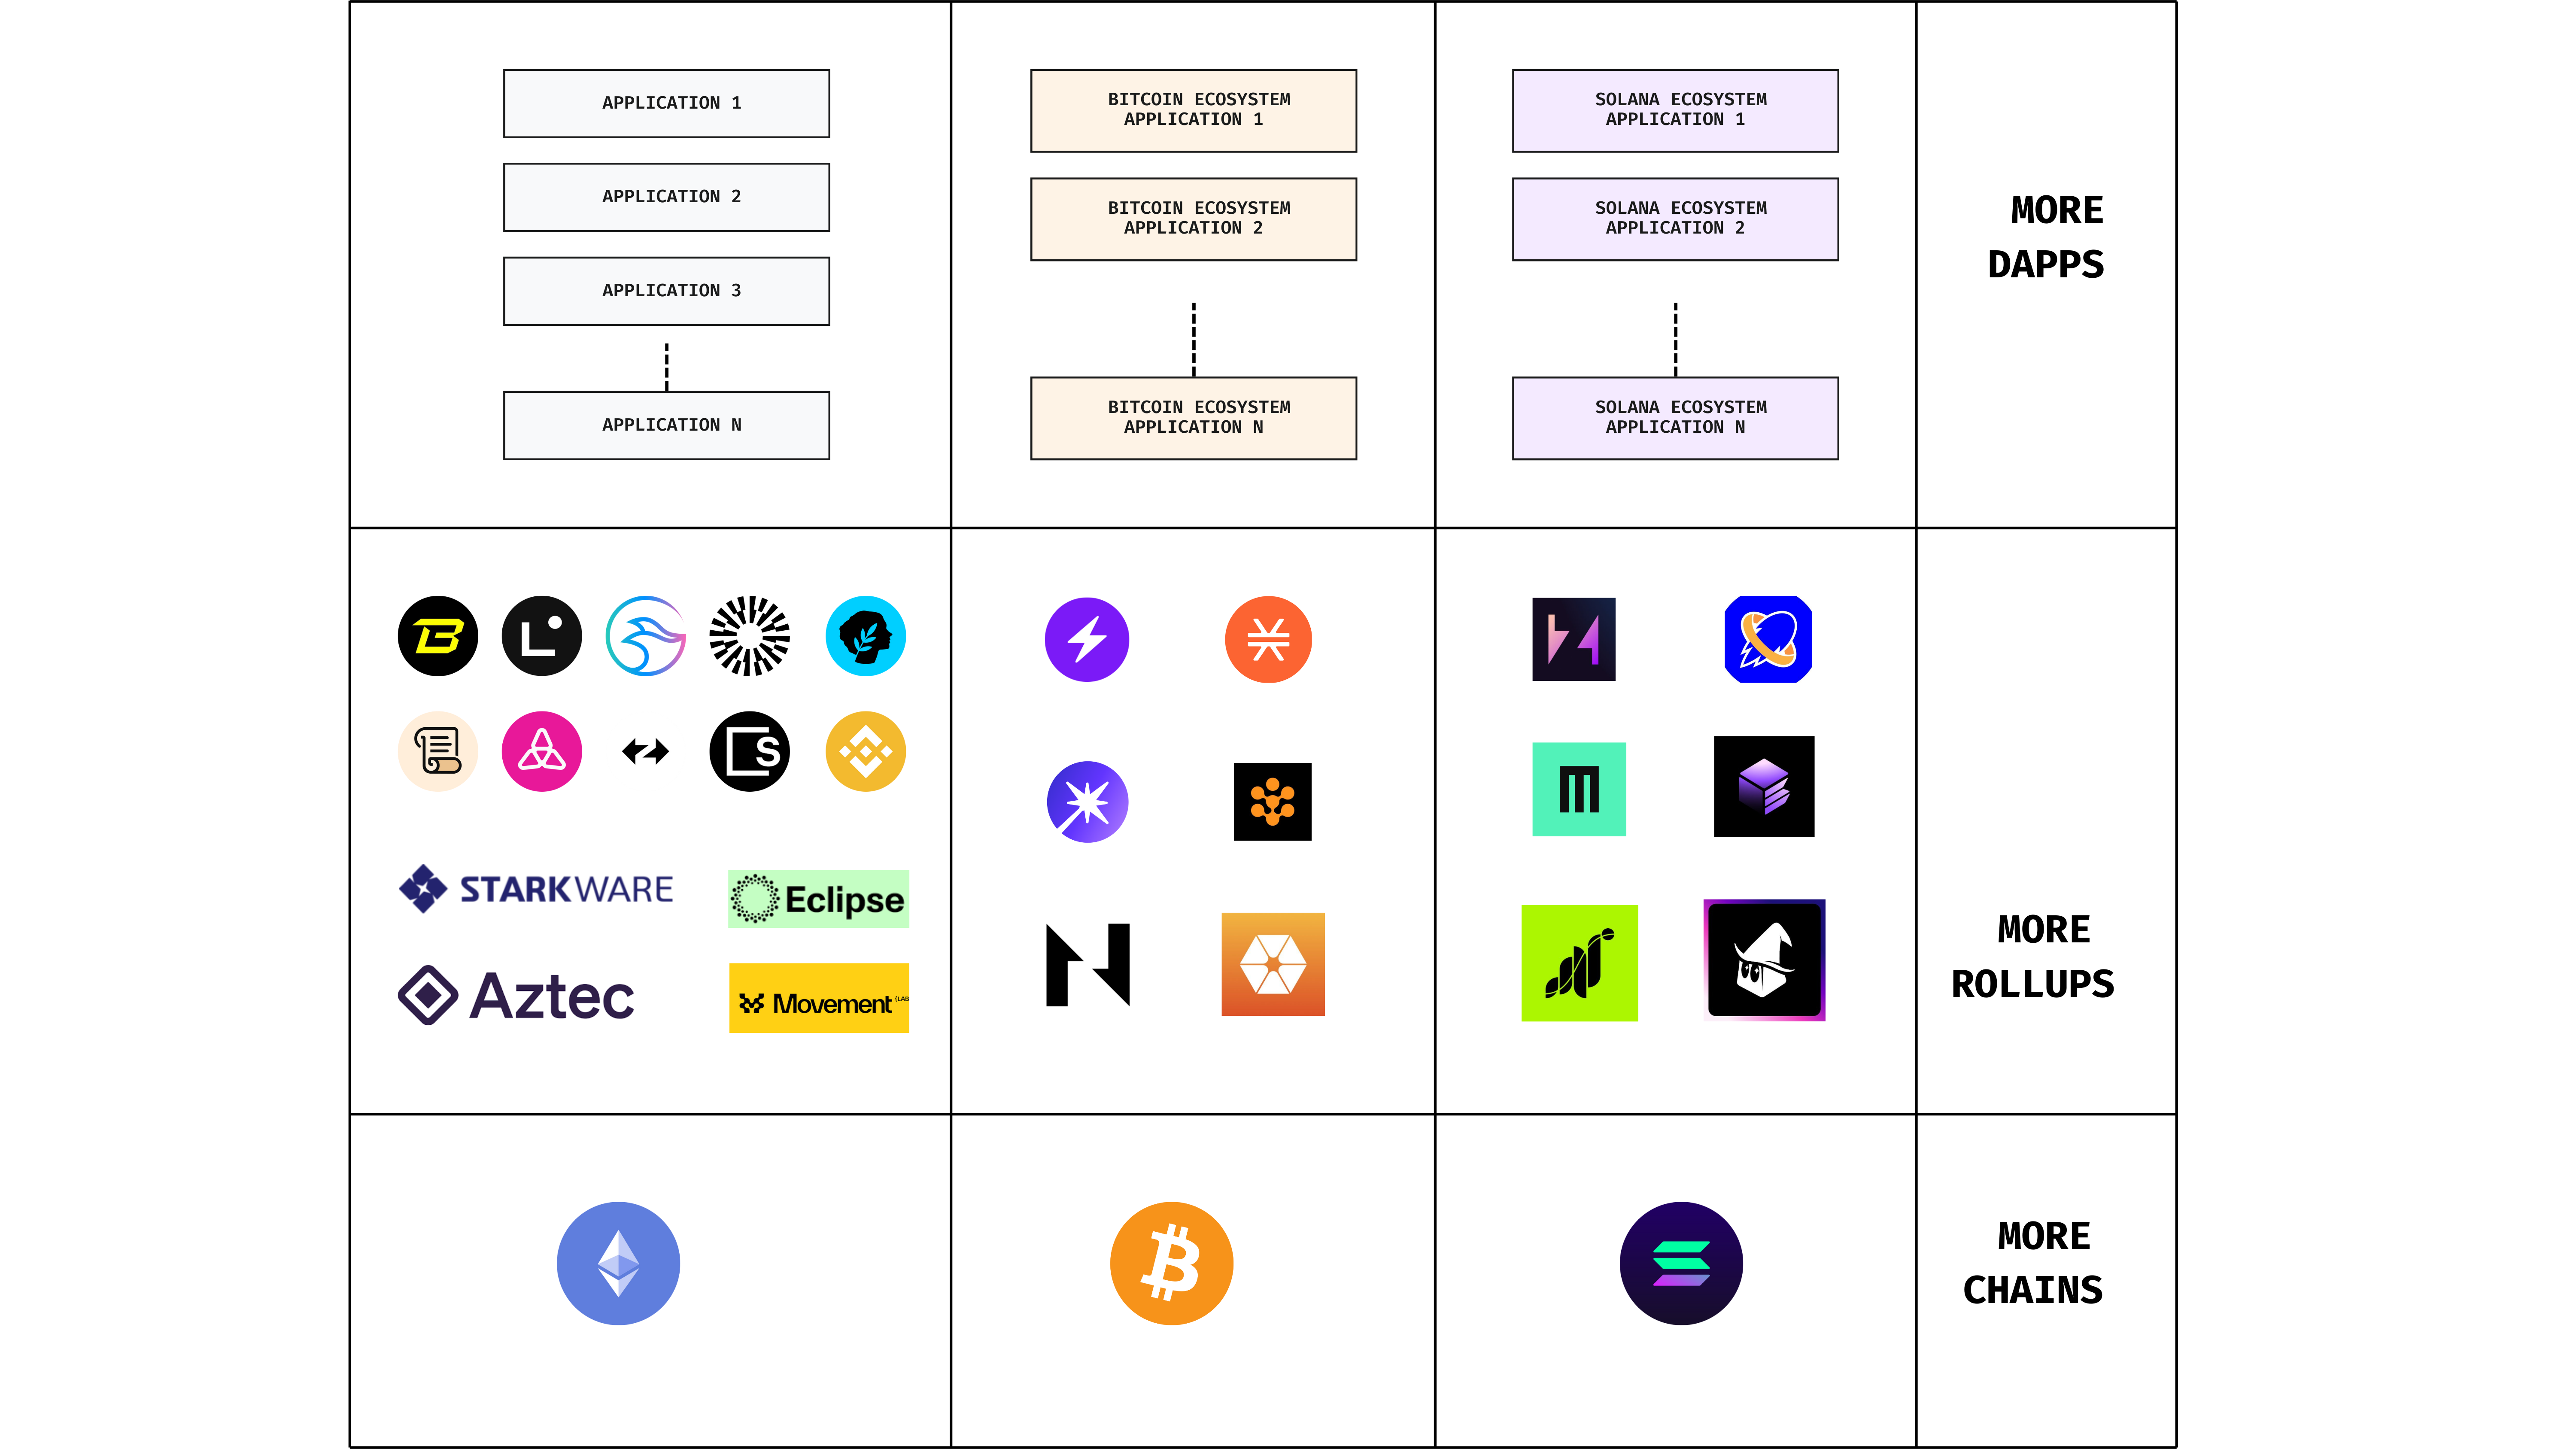
\includegraphics[width=0.99\linewidth]{figure/fragmented.png}
    \caption{Fragmented Ecosystem}
    \label{fig:fragmented}
\end{figure}


\subsection{Existing approaches}

The cross-chain ecosystem is rapidly evolving, with various solutions addressing the need for interoperability between blockchains at different layers of the stack. These solutions can generally be categorized into three key types~\cite{particle}:

1. Foundational solutions: These provide the underlying infrastructure and protocols necessary for cross-chain communication. They focus on enabling basic interoperability between chains and offering a solid foundation on which other solutions can be built.

2. Mid-level solutions: These solutions manage and coordinate cross-chain transactions and interactions. They abstract away the complexities of interoperability for decentralized applications (dApps) and ensure that data and assets can flow smoothly across different chains.

3. Comprehensive solutions: These full-stack solutions aim to cover all aspects of cross-chain interoperability, including communication, liquidity, and more. They offer broader compatibility across ecosystems and address multiple layers of interoperability in a single package. 

Each category serves a specific role in ensuring seamless communication and asset transfers between different blockchain ecosystems. However, challenges such as fragmentation and dependency bottlenecks persist, as protocols at one level depend on those beneath them. Let’s explore the existing solutions at these levels, detailing their focus areas and limitations.

\subsubsection{Foundational Solutions}

Foundational solutions focus on providing the underlying infrastructure and protocols to support cross-chain interactions. These solutions offer the base upon which other systems can build interoperability.

\textbf{LayerZero}: LayerZero~\cite{layerzero} is a protocol designed for seamless communication between heterogeneous blockchains. Specifically, it focuses on providing a universal messaging layer that can interconnect chains without restricting the system to a specific blockchain or ecosystem. Using a modular approach, LayerZero ensures that it can connect to various chains at different levels, providing a robust foundation for decentralized applications (dApps) and other protocols. The core strength of the protocol lies in its ability to facilitate trustless cross-chain messaging with minimal reliance on intermediary chains. Although LayerZero provides foundational interoperability, it still requires third-party oracles and relayers, introducing some degree of trust and centralization risk. Additionally, it does not provide solutions for handling fragmentation across ecosystems like Ethereum, Polygon, and others.

\textbf{Axelar Network:} Axelar~\cite{axelar} offers cross-chain messaging solutions that connect different blockchains in a decentralized manner. The network uses a unique approach to ensure that cross-chain transactions are routed securely, making it easier for dApps to interact across ecosystems without worrying about the underlying complexities. The key focus of Axelar is to provide a simple and unified solution that ensures a seamless experience for developers and users alike. Although Axelar supports several blockchains, its focus has been primarily on bridging Ethereum and Cosmos ecosystems, limiting the scope in terms of interoperability with other non-Cosmos- or Ethereum-based chains. Furthermore, Axelar faces scalability challenges, as it scales to support a wider variety of chains.

\textbf{Thorchain:} Thorchain~\cite{thorchain} is a decentralized liquidity protocol designed to allow cross-chain asset swaps. By using an innovative mechanism that does not rely on wrapped tokens, Thorchain enables native asset swaps between chains. Its focus on liquidity makes it particularly useful for decentralized finance (DeFi) applications. Thorchain’s reliance on native asset swaps could lead to scalability challenges, especially as it grows to support more chains. Its ecosystem is also largely focused on DeFi, limiting its applicability in broader cross-chain use cases.


\subsubsection{Mid-level Solutions}

Mid-level solutions facilitate the coordination and management of cross-chain transactions and interactions. These solutions typically abstract away the complexities of cross-chain operations for dApps and users.

\textbf{Agoric}: The focus of Agoric~\cite{agoric} is on enabling smart contracts for the creation of decentralized applications that can span multiple blockchains. Agoric brings together both foundational solutions and mod-level through its JavaScript-based environment for smart contract execution, targeting DeFi applications and cross-chain interoperability. It allows developers to create multi-chain smart contracts, but it still faces limitations with chains outside of the EVM ecosystem.

\textbf{Socket}: Socket~\cite{socket} is a cross-chain communication platform built for DeFi applications, enabling seamless communication across different blockchain networks. The main feature of the socket is its ability to support decentralized applications and services running on different L1 and L2 networks. However, its ecosystem is still somewhat Ethereum-centric and could face challenges as more non-Ethereum ecosystems like Move gain momentum.

\textbf{Skip}: Skip~\cite{skip} is a cross-chain protocol that simplifies the process of enabling decentralized applications to communicate across chains. Its focus is on supporting token and data transfers with minimal latency. Skip’s ability to work with both Ethereum-based and non-Ethereum chains makes it a promising option, but scaling to accommodate a wider range of L1 and L2 chains remains a key challenge.

\subsubsection{Comprehensive Solutions}

Comprehensive solutions are full-stack solutions designed to cover all aspects of cross-chain interoperability, including communication, liquidity, and more, while offering more extensive compatibility across ecosystems.

\textbf{Arbitrum}: Arbitrum~\cite{arbitrum} is a Layer 2 scaling solution for Ethereum that leverages optimistic rollups to improve scalability and transaction throughput. While it is primarily focused on enhancing Ethereum's scalability, it has opened up a pathway for supporting Ethereum-compatible chains and applications, making it an important player in the broader Layer 2 ecosystem. Arbitrum's focus on Ethereum means that it is limited in its ability to facilitate cross-chain interoperability outside of the Ethereum ecosystem. Furthermore, with multiple rollups being developed for Ethereum, fragmentation within the Ethereum ecosystem could increase as more L2 solutions are deployed, each with their own interoperability protocols and standards.

\textbf{Omni Network}: Omni Network~\cite{omni} offers cross-chain interoperability solutions at the Layer 2 level. It provides interoperability for various rollups and Layer 2 chains built on Ethereum. By using a robust messaging protocol, Omni Network can facilitate seamless interaction between different Ethereum-based Layer 2 solutions. Like many other Ethereum-centric solutions, Omni Network's focus remains limited to Ethereum-based ecosystems. As Ethereum rollups proliferate, the fragmentation of standards and protocols will complicate cross-chain interactions even further. Additionally, Omni's solution does not address interoperability with other Layer 1 ecosystems or new emerging ecosystems like Move-based networks.

\textbf{Polygon’s AggLayer}: Polygon’s AggLayer~\cite{aggglayer} offers an L2 scaling solution with enhanced cross-chain interoperability. It aims to improve transaction throughput across various blockchains by creating aggregated layers for data and transaction processing. Despite its innovative nature, the solution still faces the challenge of dealing with interoperability between various non-Ethereum chains, especially with the growth of Move-based rollups and L2s.

\textbf{NEAR}: NEAR Protocol~\cite{near} is designed to facilitate scalability and ease of use with a strong focus on user experience. It provides cross-chain interoperability through its bridge solutions, enabling it to communicate with Ethereum and other networks. While NEAR’s ecosystem is expanding, the continued growth of non-Ethereum chains and new smart contract languages like Move pose a challenge to its scalability and interoperability in the long term.

\textbf{Optimism’s Superchain}: Optimism’s Superchain~\cite{optimisim} focuses on interoperability at the L2 level, using the Optimistic Rollup architecture to enable Ethereum scalability. The Superchain approach envisions a multichain ecosystem powered by Optimism’s scaling technology, but its reliance on Ethereum could limit its cross-chain capabilities as other ecosystems, such as Move, develop and emerge with different architectures and priorities.

\subsubsection{Bottlenecks and Dependencies Across Layers}

One of the key challenges facing the development of cross-chain interoperability is the bottleneck effect that arises from the dependency between different protocol layers. The foundational protocols rely on the security and performance of the chains they are connected to. For example, if a foundational solution like LayerZero or Axelar faces issues in communication or scalability, it could cause disruptions for higher-level  solutions like Agoric or Socket, which, in turn, would impact the overall user experience and reliability of comprehensive solutions like Polygon’s AggLayer or Arbitrum.

As each level is co-dependent on the one below, the compromise of a protocol at the foundational layer can cause cascading failures or reduced functionality across all other layers. To address this challenge, a comprehensive solution would need to work with multiple foundational protocols while mitigating the risks of fragmentation and ensuring strong cross-chain communication across all levels.

In summary, the landscape of cross-chain interoperability solutions is diverse, with foundational, mid-level, and comprehensive solutions offering different levels of integration. However, with the emergence of new ecosystems and the rise of Move-based rollups, it is clear that the industry must adapt to these changes or face further fragmentation and siloing across the blockchain space.

\subsection{Overview of the Omnichain Web} % Add a subsection

Omnichain Web stands out as a truly comprehensive solution by offering a unified framework for seamless interoperability across all blockchains, bypassing the bottlenecks that traditional solutions face. Unlike existing comprehensive solutions, which are often constrained by their reliance on specific ecosystems or foundational protocols, Omnichain Web integrates multiple L1s, L2s, and even emerging ecosystems like Move, enabling decentralized applications (dApps) to operate across the entire blockchain landscape without friction. By abstracting away the complexity of cross-chain interactions and providing a robust layer of universal communication, Omnichain Web eliminates the cascading failures that occur when one layer encounters issues. This holistic approach ensures that the infrastructure remains secure, scalable, and future-proof, allowing developers to focus on innovation without worrying about fragmentation or dependency on a single ecosystem. With Omnichain Web, blockchain interoperability is no longer a challenge but a seamless and reliable experience for both developers and users alike.

\begin{figure}[h]
    \centering
    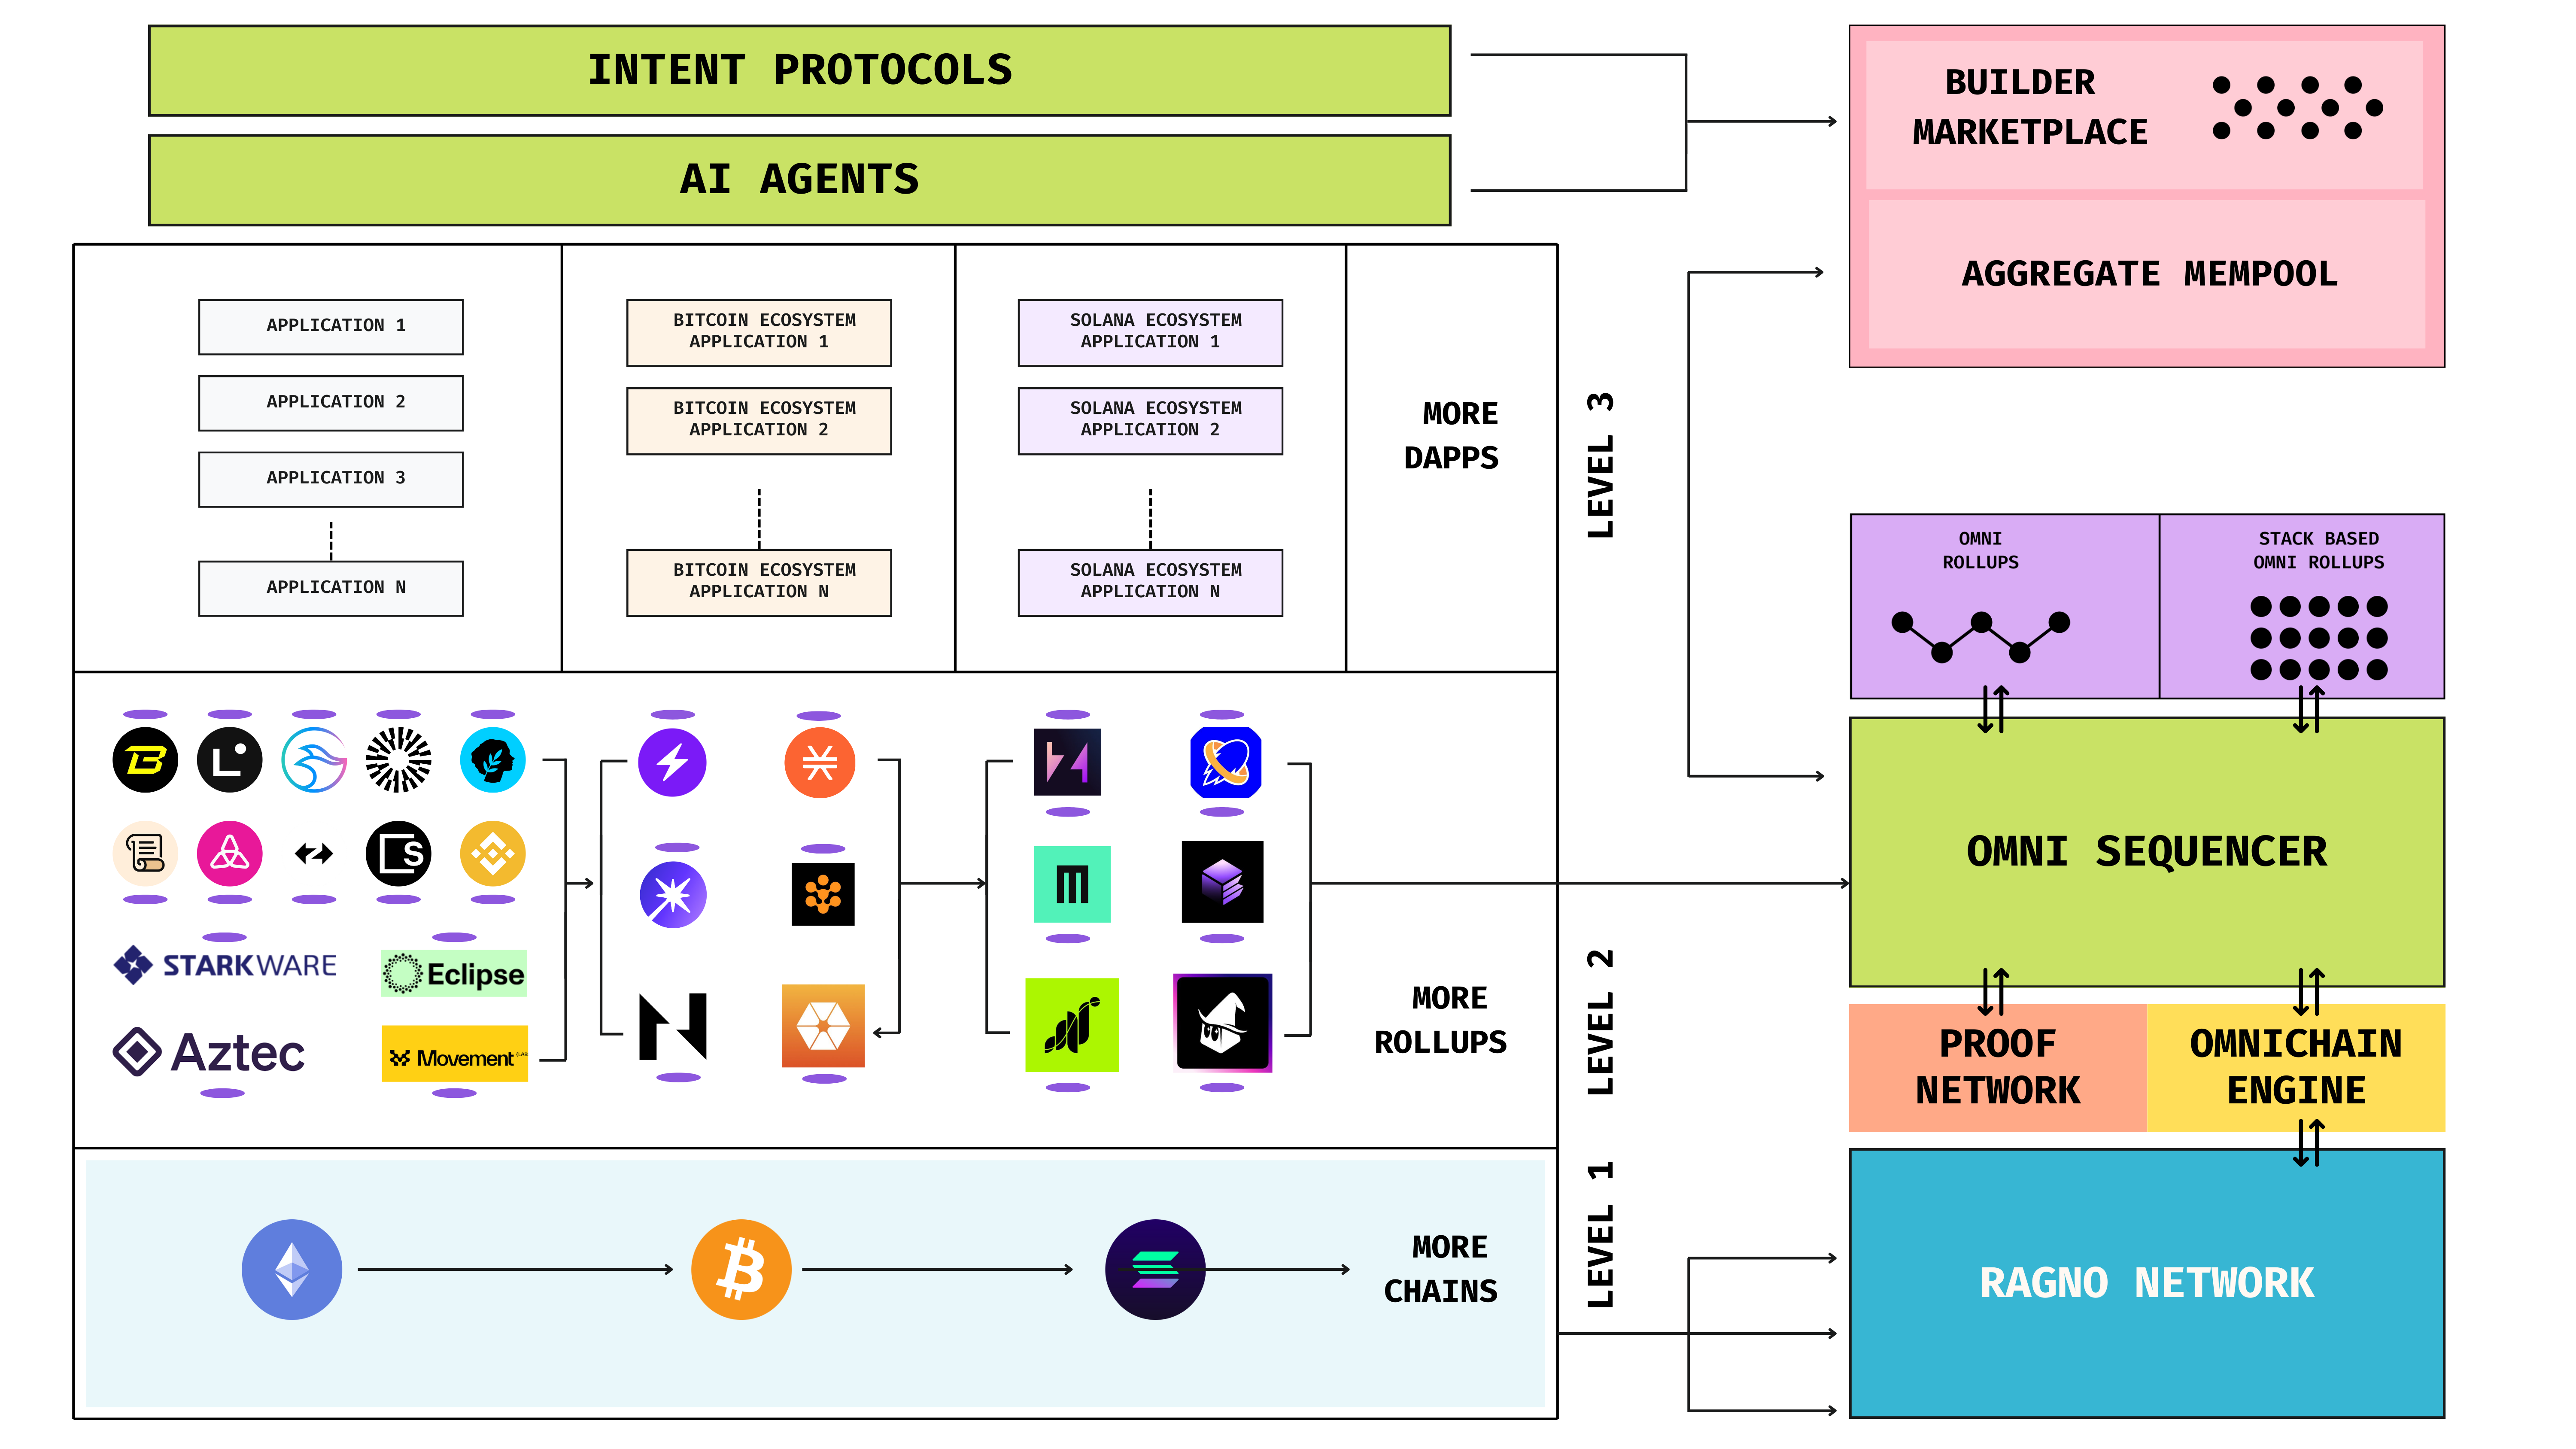
\includegraphics[width=0.99\linewidth]{figure/connected.png}
    \caption{Connected Ecosystem}
    \label{fig:connected}
\end{figure}

The Omnichain Web consists of four core components: Builder Marketplace, Omni Sequencer, Prover Network, and Ragno Network. Each part plays a distinct role in ensuring efficient, secure, and interoperable operations across the ecosystem.

\begin{itemize}
    \item[1.] \textbf{Builder Marketplace}

%The Builder Marketplace serves as the ecosystem's application layer, hosting decentralized applications (dApps) and solvers that are deployed in Trusted Execution Environments (TEE) for enhanced integrity and security.

The Builder Marketplace is responsible for unifying protocols from all chains into structured modules, enabling developers to build customized solvers with cross-communication capabilities. It supports universal transaction flows from intent-centric apps, AI agents, and direct API calls, ensuring seamless interoperability and efficiency.

Features:
    \begin{itemize}
        \item Applications such as AI Agent and Intent Protocol enable users to submit inputs for processing.
        \item Users can interact with solvers through multiple interfaces, such as customized frontends, AI agents, TEE environments, or by directly utilizing solver API endpoints.
        \item Solvers process inputs and produce optimized transaction batches for further processing.
    \end{itemize}

    \item[2.] \textbf{Omni Sequencer}

The Omni Sequencer is responsible for aggregating and organizing transactions from solvers, rollups, or direct user submissions.

Functionality:
    \begin{itemize}
        \item Receives transactions via a sequencer client and bundles them into blocks based on settlement chains.
        \item Orders transactions and generates commitments to the ordering.
        \item Publishes commitments to a Data Availability (DA) layer or smart contract.
        \item Sends blocks to the rollup executor for execution and settlement.
    \end{itemize}
    

    \item[3.] \textbf{Prover Network}

The Prover Network underpins the ecosystem’s cryptographic security by providing proofs for state transition functions.

Key Features:
    \begin{itemize}
        \item Distributed Jolt-based zkVM for generating computational proofs.
        \item Utilizes the Binius proof system, optimized for binary operations critical to machine computations.
        \item Generates proofs for rollup state transitions, ensuring the validity of updates before they are sent to settlement chain contracts.
    \end{itemize}
    

    \item[4.] \textbf{Ragno Network}

The Ragno Network ensures robust data aggregation and transaction validation through its operators and Hermes Chain. The settlement process involves pre-confirmation on the Hermes Chain and verification of source chain execution before finalizing on the target chain.

Components:
    \begin{itemize}
        \item Operators: Nodes registered on the Hermes chain, responsible for fetching and processing blocks from different chains.
        \item Crawler: Maintains an updated list of operators and filters blocks for transactions related to Dojima Chain.
        \item Hermes: Publishes filtered transactions on the Hermes Chain and processes them.
        \item Narada: Signs outbound transactions using GG20 TSS and passes them to the respective rollup for execution, with additional verification by the Crawler. 
    \end{itemize}
    
\end{itemize}  
%

\section{Preliminaries}


\subsection{Threshold Signature Scheme (TSS)}

\subsection{Tendermint}

\subsection{Jolt zkVM}




\section{Transaction Abstraction }

An abstract transaction is a generalized representation of a blockchain transaction that abstracts away the specific details of any particular blockchain protocol. It provides a standardized format for encapsulating all necessary information required for transaction execution, such as sender/receiver addresses, transaction data, gas limits, proofs, and other metadata. This abstraction ensures that transactions can be processed seamlessly across different blockchain networks, regardless of their underlying protocols, consensus mechanisms, or data structures. In simpler terms, an abstract transaction is a unified language that bridges the differences between blockchains, enabling communication and interaction across multiple networks.


An abstract transaction in the Omnichain ecosystem is designed to carry all the necessary information for cross-chain execution. The following is a detailed format:
\begin{itemize}
    \item \textbf{Header:}
    The header contains metadata about the transaction:
    \begin{itemize}
        \item \textsf{Transaction ID}: Unique identifier for the transaction.
        \item \textsf{Source Chain ID}: Identifier of the chain from which the transaction originates.
        \item \textsf{Target Chain ID(s)}: Identifier(s) of the destination chain(s).
        \item \textsf{Nonce}: A unique number to ensure transaction uniqueness and prevent replay attacks.
        \item \textsf{Timestamp}: Time of transaction creation for ordering and validation.
    \end{itemize}
    \item \textbf{Payload:}
    The payload includes the core logic and data of the transaction:
    \begin{itemize}
        \item \textsf{Sender Address}: Address of the user or entity initiating the transaction.
        \item \textsf{Receiver Address}: Target address on the destination chain.
        \item \textsf{Action Type}: Specifies the transaction type (e.g., transfer, invocation of smart contracts).
        \item \textsf{Data/Call Parameters}: Encoded data required to execute the action on the target chain (e.g., function arguments for contract calls).
        \item \textsf{Asset Details (if applicable)}:\\
            Asset ID: Token or asset being transferred.\\
            Amount: Quantity of the asset being transferred.
    \end{itemize}

    \item \textbf{Execution Details:}
    Information about the execution context:
    \begin{itemize}
        \item \textsf{Gas Limit}: Upper limit for gas usage (abstracted from the user, automatically handled by the system).
        \item \textsf{Fee Payment Details}: Specifies how fees are handled, such as being paid in native tokens or abstracted through relayers.
        \item \textsf{Batch Information}: Indicates if the transaction is part of a batch (used for solver optimization).
    \end{itemize}

    \item \textbf{Proofs and Signatures:}
    Cryptographic elements to ensure validity and security:
    \begin{itemize}
        \item \textsf{Source Chain Proof}: Proof confirming execution on the source chain.
        \item \textsf{Cross-Chain Proof}: Generated by the Prover Network for the state transition function.
        \item \textsf{Signatures}: Cryptographic signatures from the sender or relayer for authorization.
    \end{itemize}

    \item \textbf{Settlement Instructions:}
    Instructions for final settlement:
    \begin{itemize}
        \item \textsf{Target Contract Address}: Smart contract on the destination chain to execute the transaction.
        \item \textsf{Confirmation Requirement}: Specifies whether the execution of the source chain must be confirmed before settlement.
        \item \textsf{Rollback Mechanism}: Conditions and actions to handle failed transactions.
    \end{itemize}
\end{itemize}

 

    

  


\section{Core Components}







 
\subsection{Omnichain Engine}

The Omnichain Engine is a powerful interoperability framework built on the Hermes chain, with the Narada Service providing secure key management and execution support. Using the Tendermint consensus protocol for block creation, ensuring high-speed finality, Byzantine fault tolerance (BFT) and efficient transaction processing. Tendermint’s~\cite{tendermint} consensus mechanism is designed to provide fast block confirmation while maintaining security, making it ideal for cross-chain communication and decentralized execution.

At the core of the Omnichain Engine, the Hermes chain functions as the primary coordination layer, managing cross-chain transactions, state updates, and message passing between different rollups and blockchain networks. It ensure that cross-chain operations are executed efficiently and securely, serving as the backbone of the omnichain ecosystem.

\begin{figure}[h]
    \centering
    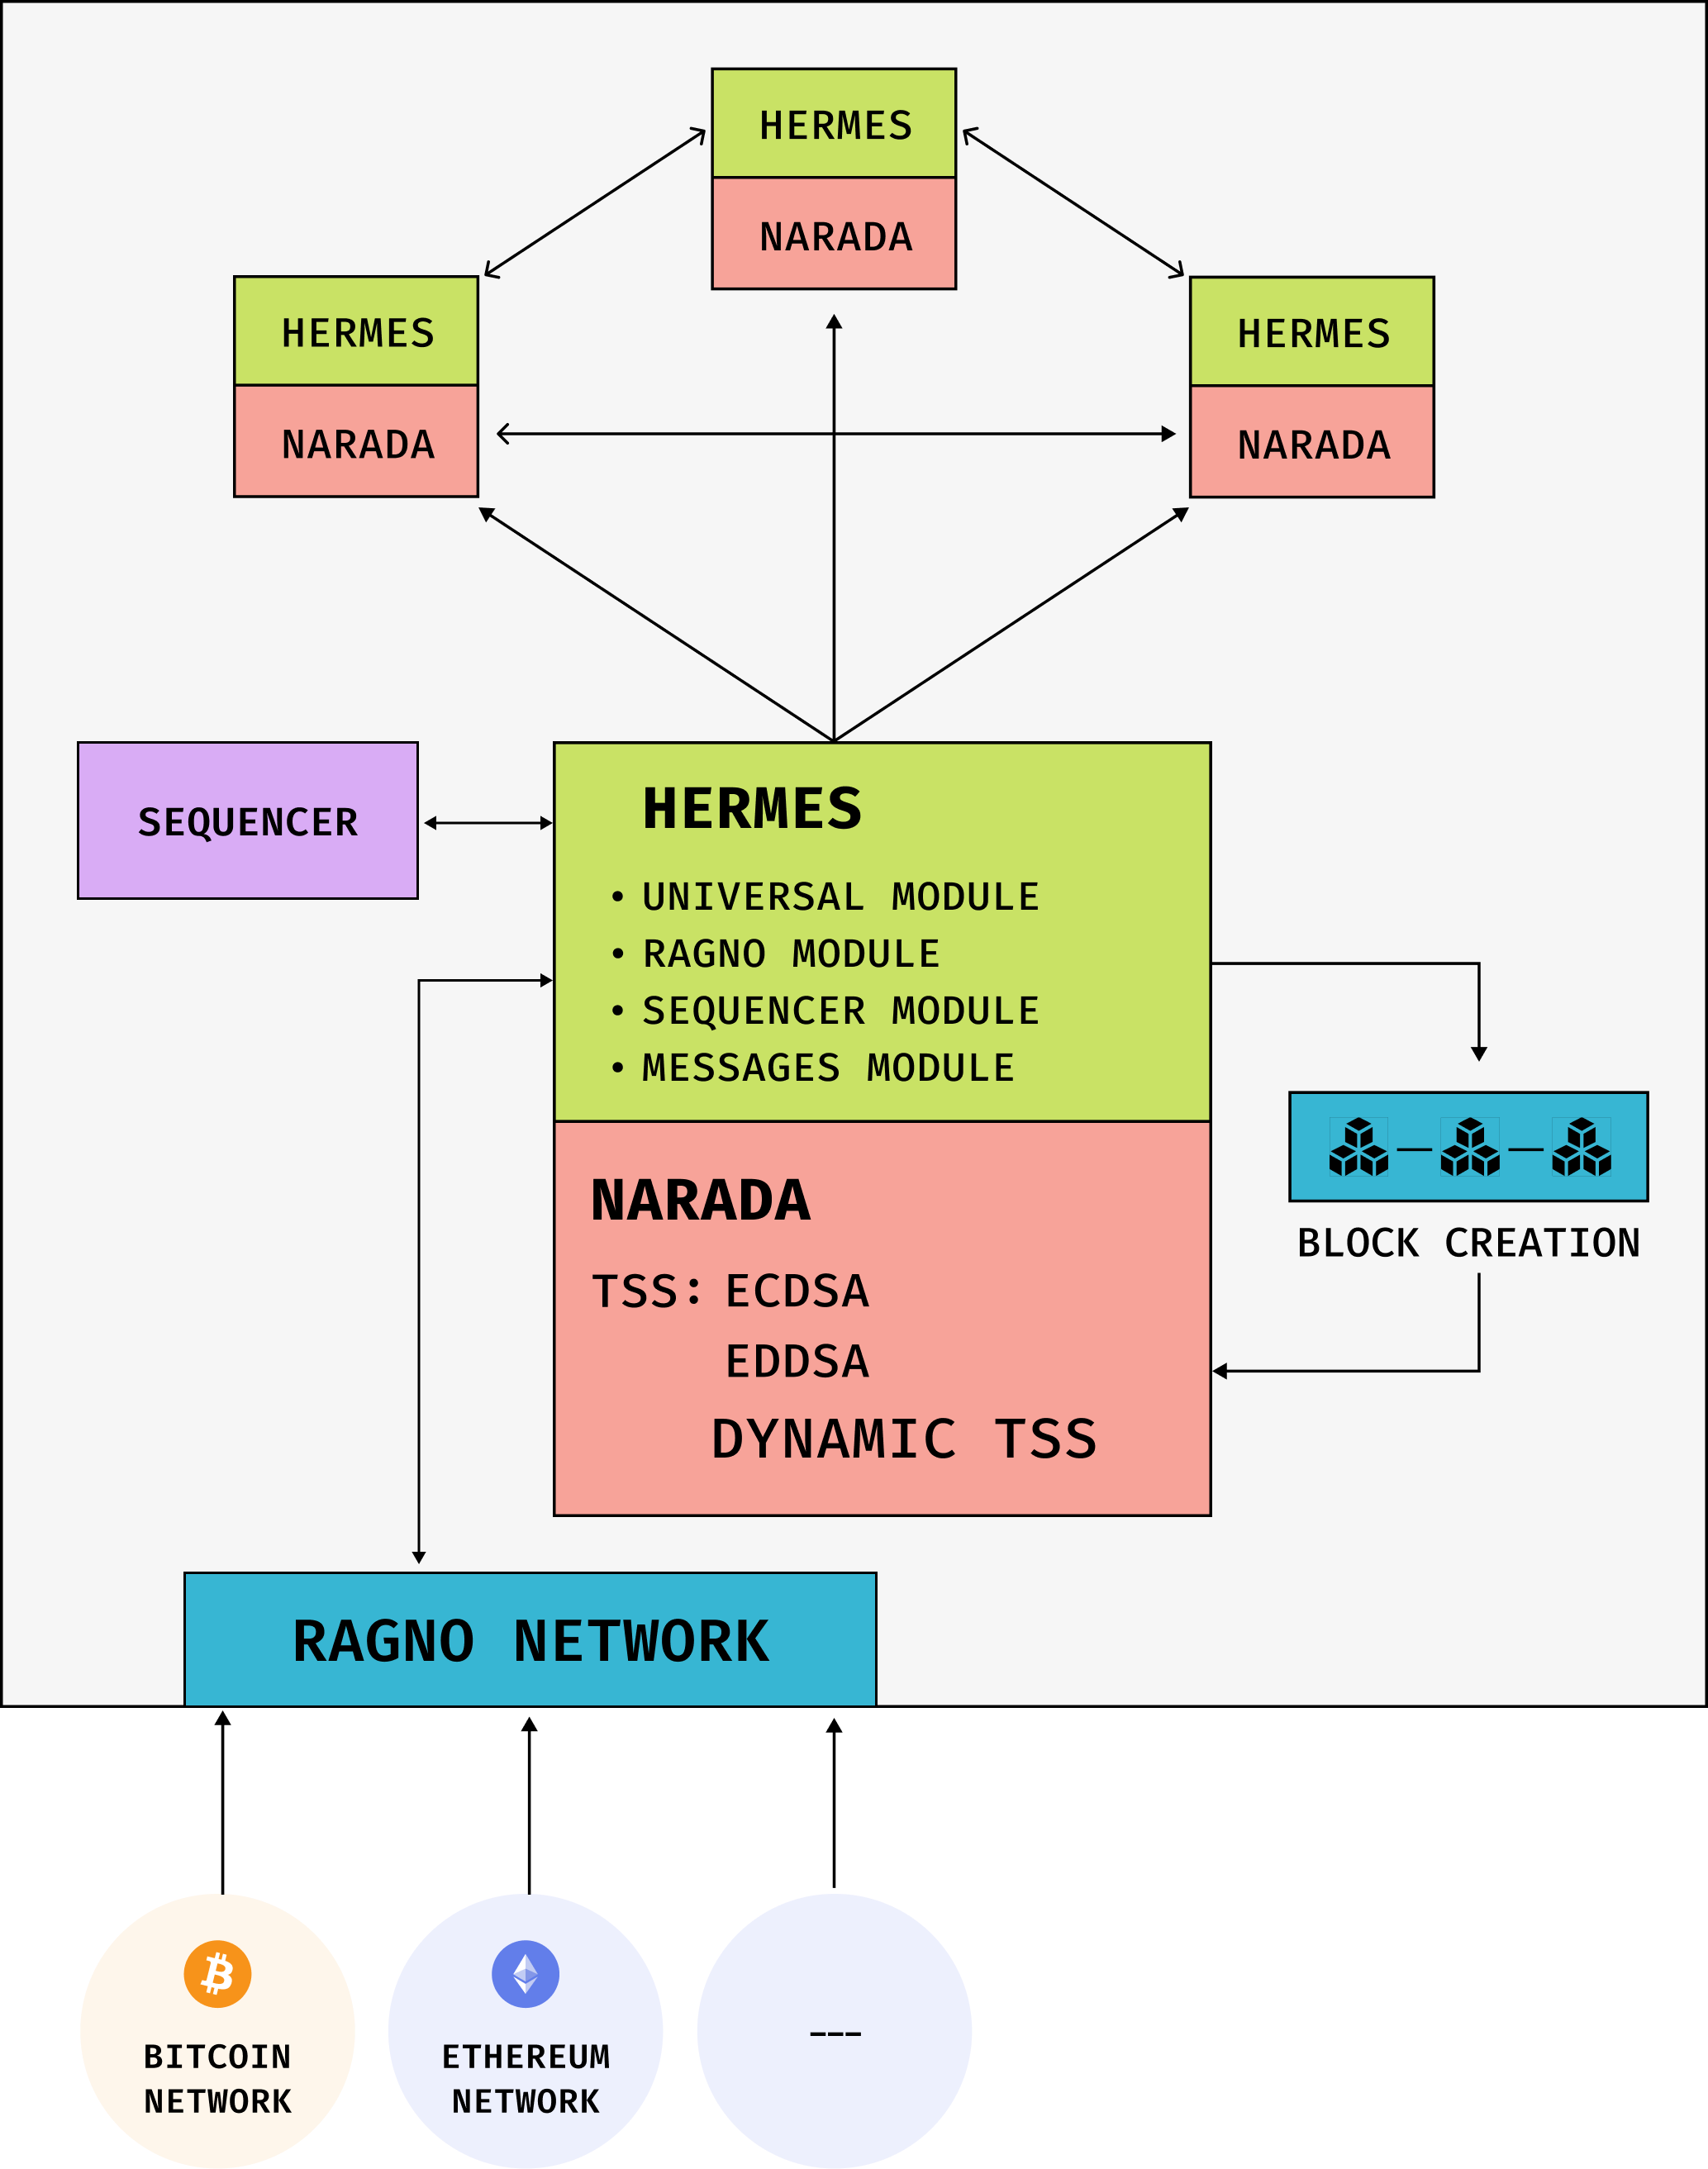
\includegraphics[width=0.7\linewidth]{figure/engine.png}
    \caption{Omnichain Egine}
    \label{fig:engine}
\end{figure}

A critical component of this architecture is the Narada Service, which provides the CGGMP Threshold Signature Scheme (TSS)~\cite{tss} functionality, enabling decentralized key management. This allows the Omnichain Engine to control and sign transactions for any addresses it manages without relying on a single point of failure. Furthermore, Narada extends TSS support to addresses controlled by private rollup clients, enabling enterprises and customized rollup solutions to securely manage cross-chain assets and operations.

By combining Tendermint’s fast and secure consensus, Hermes Chain’s interoperability capabilities, and Narada Service’s decentralized key management, the Omnichain Engine creates a trustless, scalable, and flexible environment for cross-chain transactions. This architecture empowers developers to build omnichain applications with seamless connectivity, robust security, and efficient execution.


\subsubsection{Threshold Signature Scheme (TSS)}

The cggmp TSS~\cite{tss} Scheme enables a distributed set of participants to collaboratively generate and use a cryptographic key for secure signing without having full control. The scheme consists of three key phases: \textsf{Key Generation}, \textsf{Pre-Signing}, and \textsf{Signing}, with an additional \textsf{Key Refresh} mechanism to maintain security over time.  

\begin{itemize}
    \item \textbf{Key Generation}
    
    Upon receiving the input (\textsf{keygen}, \textsf{sid}, $i$), the system initializes the key setup process:  
    \begin{itemize}
        \item[1.] Executes the key generation phase, obtaining the partial secret share $X_0$ and the public key $\textsf{pk}$.  
        \item[2.] Runs the auxiliary information phase, processing (\textsf{aux-info}, \textsf{sid}, $X_0$, $i$) to output essential parameters: $(\textsf{sid}, \textsf{rid}, X^*, N, s, t)$ and individual participant-specific values $(x_i, y_i, p_i, q_i)$.  Assigns an epoch identifier (\textsf{epid}) to encapsulate these parameters:  
     \[
     epid = (\textsf{sid}, \textsf{rid}, X^*, N, s, t)
     \]
        \item[3.] Outputs the public key $\textsf{pk}$ associated with the session identifier \textsf{sid}.  
    \end{itemize}

    \item \textbf{Pre-Signing} 
    
    To prepare for signing, the system processes the input $(\textsf{pre-sign}, \textsf{epid}, L, i)$:  
    \begin{itemize}
        \item[1.] Erases all previous presigning data associated with \textsf{epid} to maintain security.  
        \item[2.] Runs the pre-signing phase concurrently for all $l\in [L]$, initializing multiple pre-signing sessions.  
        \item[3.] Once presigning is completed, the system remains on standby, awaiting the actual signing request.  
    \end{itemize}

    \item \textbf{Signing}
    
    When a signature is requested for a message \textsf{msg}, the system processes $(\textsf{sign}, \textsf{epid}, \textsf{sgid}, l, i, \textsf{msg})$ as follows: 
    \begin{itemize}
        \item[1.] Converts the message \textsf{msg} into a standardized form $m = F(\textsf{msg})$.  
        \item[2.] Runs the signing phase with input $(\textsf{sign}, \textsf{epid}, \textsf{sgid}, l, i, m)$ to generate a signature $\sigma$ and a verification set $Q$:  If $\sigma$ is valid, $Q = \phi$. Otherwise, $Q$ contains the identifier of a detected corrupted party.  
        \item[3.] Outputs the signature tuple:  
   \[
   (\textsf{sig-string, sid, sgid, msg}, \sigma, Q)
   \]  
    \end{itemize}

    \item \textbf{Key Refresh}  
    
    To refresh cryptographic keys, the system processes $(\textsf{key-refresh, sid}, X, i)$, ensuring continued security and integrity.  
    \begin{itemize}
        \item[1.] Runs the auxiliary information phase on $(\textsf{aux-info, sid}, X, i)$.  
        \item[2.] Retrieves updated parameters $(\textsf{sid, rid}, i, X^*, N, s, t)$ along with participant-specific values $(x_i, y_i, p_i, q_i)$.  
        \item[3.] Erases all previous presigning and auxiliary information related to the prior \textsf{epid}.  
        \item[4.] Assigns a new \textsf{epid}:  
   \[
   epid = (\textsf{sid, rid}, X^*, N, s, t)
   \]
        \item[5.] If an error occurs during the refresh process, all future key-refresh operations for this session are ignored to prevent inconsistencies.  
    \end{itemize}

\end{itemize}

The auxiliary information phase runs the secret sharing scheme for $0$ and adds these shares to the shares of the secret key $\textsf{sk}$. This gives new secret shares for the secret key. The TSS framework provides secure, fault-tolerant multi-party signing, ensuring privacy and resilience against adversarial actions while maintaining decentralized control.




\subsection{Ragno Network}

The Ragno Network serves as the foundational layer of the Omnichain Web and emerged from a personal challenge we encountered with the initial V1 of the Dojima architecture. This is a challenge common to all cross-chain protocols, where adding a new chain requires each validator to either run a new node or update their RPC URLs—both costly and complex tasks. The Ragno Network is a cutting-edge protocol designed for interoperability between Layer 1 (L1) blockchains. It addresses key issues that hinder seamless interaction and communication across different blockchain ecosystems. By addressing fragmentation and inefficiencies in cross-chain operations, Ragno plays a crucial role in enabling interconnectedness, scalability, and security within decentralized networks. Its innovative architecture is central to the ongoing evolution of blockchain technology.

Ragno eliminates the need for centralized intermediaries by utilizing a decentralized protocol driven by a network of validators and relayers. This ensures that all cross-chain operations are trustless, resilient, and aligned with the core principles of decentralization. At the heart of the network is a universal messaging layer that facilitates seamless communication between L1 chains. Through this layer, arbitrary data, assets, and state information can be securely and efficiently transferred between chains. Ragno enhances its security framework with multisignature schemes, fraud proofs, and dynamic validator sets, ensuring that only valid transactions are executed and protecting the network from malicious activities.

Ragno’s design prioritizes both compatibility and scalability. The protocol is adaptable to account-based and UTXO-based blockchain architectures, allowing it to integrate with a wide range of existing and emerging technologies. In addition, Ragno supports a developer-friendly ecosystem by providing robust APIs, SDKs, and comprehensive documentation. This empowers developers to build cross-chain-enabled decentralized applications (dApps) efficiently, accelerating the adoption of interoperable blockchain solutions.
\subsubsection{Core Protocol Design} 

The Ragno Network is a critical part of the Omnichain ecosystem, responsible for data aggregation, validation, and secure communication across multiple blockchain networks. It consists of the following main components:

\begin{itemize}
    \item \textsf{Operators :} Operators are nodes that play a vital role in the Ragno network by facilitating the flow and validation of transactions. Anyone running a node on a blockchain network can become an operator by registering it on the Hermes Chain. Operators fetch and relay blocks or transactions from their respective chains to the Ragno network. Operating under decentralized principles, they ensure robust and fault-tolerant operations by eliminating any single point of failure.
    \item \textsf{Hermes Chain :} The Hermes chain functions as the coordination layer of the Ragno network, playing a pivotal role in ensuring seamless operations. It maintains an updated registry of active operators by receiving periodic updates from the Crawler component. Serving as a decentralized ledger, it records pre-confirmations of cross-chain transactions, providing an additional layer of transparency and reliability. Furthermore, the Hermes Chain tracks and processes transactions from their source to target chains, ensuring consistency and integrity throughout the cross-chain communication process.
    \item \textsf{Microservices :} The Ragno Network operates through three specialized microservices that perform distinct roles:
    \begin{itemize}
        \item \textsf{Crawler :} The Crawler continuously updates the registry of active operators by querying the Hermes Chain at regular intervals. It also filters blocks retrieved by operators, isolating transactions relevant to specific chains, such as the Dojima chain, to ensure accurate and efficient processing.
        \item \textsf{Hermes :} Hermes processes filtered transactions received from the Crawler, publishes preconfirmations on the Hermes Chain to track pending cross-chain transactions, and manages transaction routing while preparing the transactions for execution on the target chain.
        \item \textsf{Narada :} Narada manages outbound transactions by signing them with the CGGMP protocol~\cite{tss}, a dynamic threshold signature scheme (TSS), ensuring robust cryptographic security. It verifies that all transactions are securely signed before forwarding them to the target rollup or chain for execution. Narada collaborates with the Crawler to validate the signatures, providing an additional layer of assurance prior to final execution.
    \end{itemize}
\end{itemize} 

A user, Intent protocol or AI agent initiates a transaction request through the Builder Marketplace or directly within the ecosystem. This transaction is abstracted into a standardized format, encapsulating essential details such as the source chain, the target chain, and the payload. The network of clients, in collaboration with operators, will be responsible for fetching transactions. Operators will retrieve native system addresses, while individual clients will fetch transactions specific to the OmniRollup or user applications. These transactions will then be reported to crawlers for processing. The crawlers will process these blocks, extracting transactions relevant to the target chain. 

\begin{figure}[h!]
    \centering
    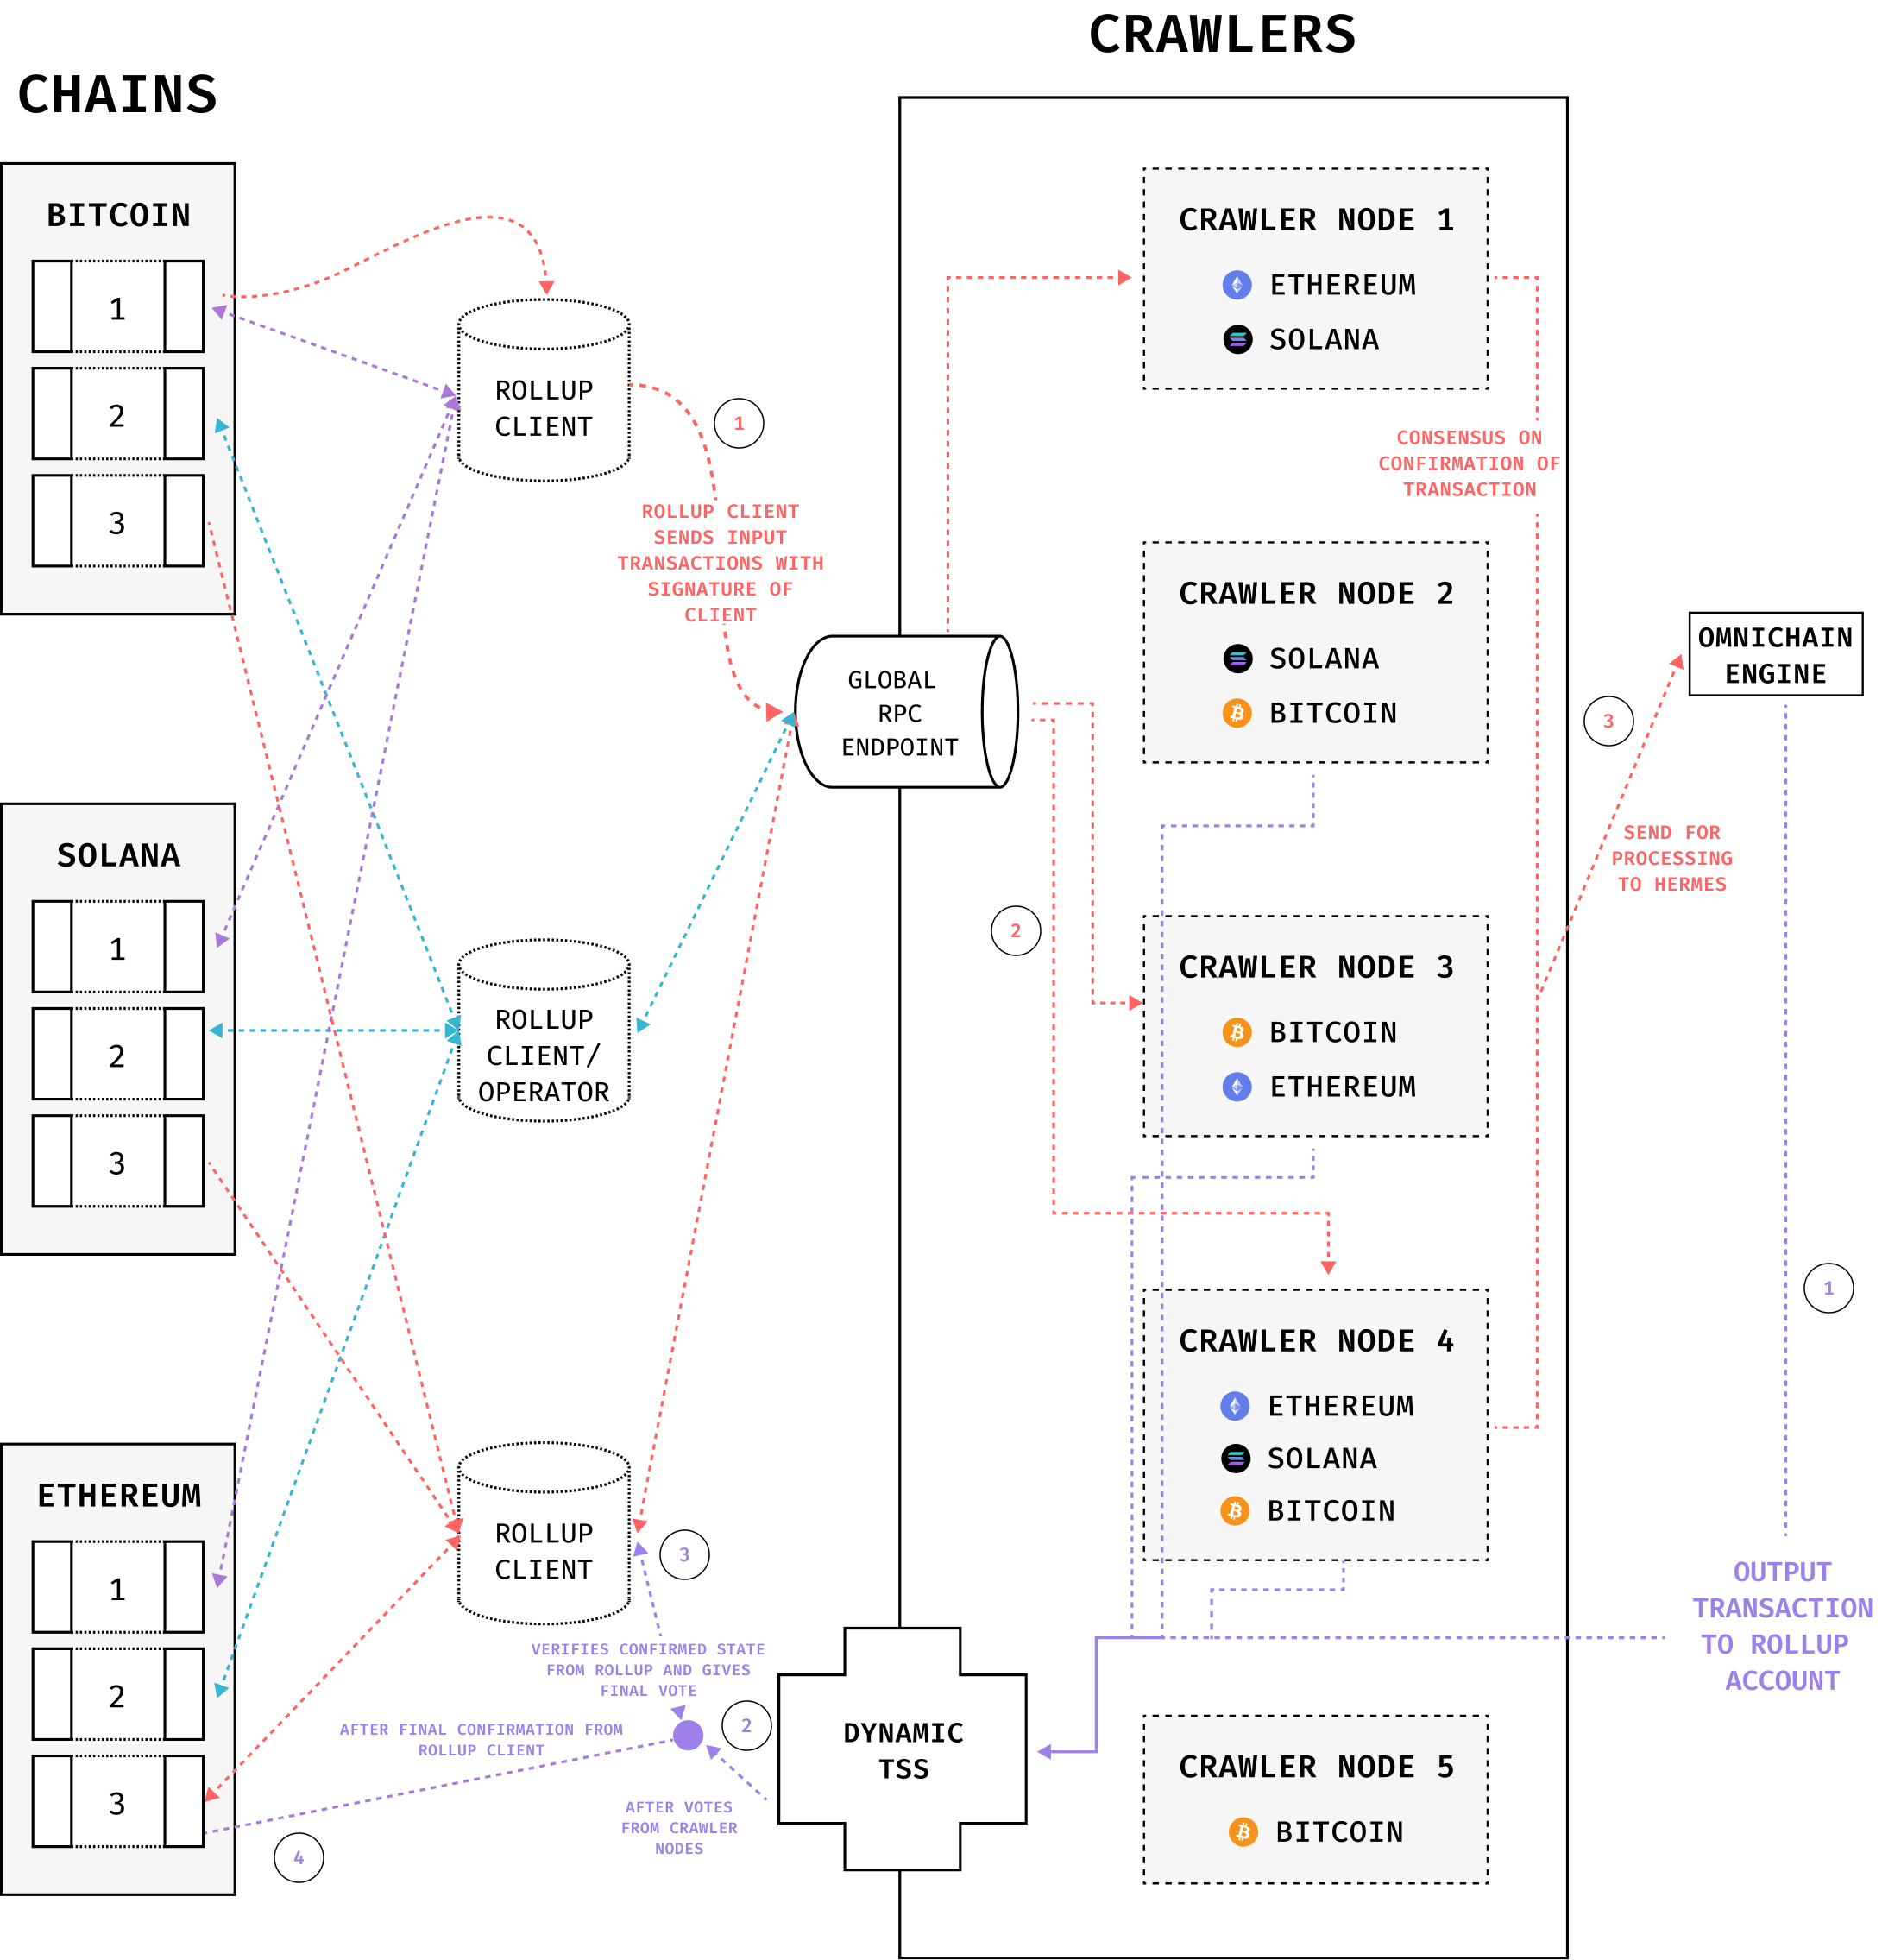
\includegraphics[width=0.99\linewidth]{figure/ragno.png}
    \caption{Ragno Network Overview}
    \label{fig:ragno}
\end{figure}

The Hermes microservice publishes these filtered transactions as preconfirmations on the Hermes chain, which acts as a checkpoint to ensure that the transactions have been identified and validated for further processing. Block creation is governed by the Tendermint consensus protocol, which requires consensus among crawlers. An incoming transaction is recorded only when a majority of Crawlers receive identical transaction data from different operators.  

Before settlement, the protocol confirms that the corresponding transaction on the source chain has been successfully executed. This verification is achieved by cross-referencing the transaction’s status on the source chain, either using a proof generated by the Prover Network or through a direct query via Hermes.

The Narada microservice monitors outbound transactions destined for the target chain. These transactions are signed using the GG20 threshold ECDSA Signature Scheme (TSS), ensuring cryptographic security and resilience against single points of failure. After signing, the transactions are verified by the crawler to ensure integrity. Once validated, they are forwarded to the target chain for settlement. The target chain executes the transaction and updates its state based on the provided payload.

Upon successful execution on the target chain, the Hermes chain records the transaction's final state. This record is updated to reflect the successful completion of cross-chain communication and settlement, thus completing the transaction lifecycle.

\subsubsection{Operator Registration}

The registration process for operators in the Ragno network ensures a secure and decentralized mechanism to accept participants who play a critical role in maintaining cross-chain communication. The first step involves staking \$DOJ tokens, a requirement that aligns operator incentives with the goals of the network. Operators use the `\textsf{createOperator}` functionality to stake the tokens, which not only secures their participation but also adds them to the set of operators maintained on the Hermes chain. This stake mechanism guarantees commitment and mitigates malicious behavior within the ecosystem.  

Once onboarded, operators are required to host blockchain nodes of their chosen networks. These nodes facilitate the relay and validation of transactions across chains. Operators manage and register their nodes via the Operator Dashboard, which serves as a centralized interface for updating and maintaining their infrastructure. Any changes or additions to the nodes are automatically recorded in the Hermes chain through the dashboard, ensuring transparency and up-to-date records.  

To maintain synchronization and efficiency, crawler nodes continuously monitor the Hermes chain for operator-related events, such as updates to the operator set or node configurations. These events are filtered and stored locally by crawlers, enabling rapid querying and reducing overhead during data synchronization. This robust monitoring mechanism ensures that the Ragno network is up-to-date with the latest operator and node information, providing a reliable backbone for cross-chain communication.

\subsubsection{Data Fetching Process}
The data fetching process in the Ragno Network employs a structured, secure, and pull-based mechanism to ensure efficient and authenticated communication between crawler nodes and operator nodes. This process is based on the Hermes chain, which plays a central role in managing mappings, ensuring fairness, and maintaining the integrity of the data flow.

\textbf{Pull-Based Mechanism and Pairing List (PL)}

The crawler nodes operate on a pull-based system, periodically querying the operator nodes to retrieve the latest blockchain data. To coordinate these interactions, the Hermes Chain publishes a Pairing List (PL) every 200 blocks. The PL assigns specific crawler nodes to designated operator nodes, defining which crawlers are responsible for fetching data from which operators. This mapping ensures an equitable distribution of workload across the network and prevents unnecessary redundancies.

The PL is aggregated based on submissions from crawlers, finalized on the Hermes Chain, and then disseminated to all crawler nodes. Crawlers use this final PL to determine their assigned operator and initiate data requests. Crawlers can only fetch data from operators they are mapped to, ensuring strict adherence to PL guidelines and preventing unauthorized data access.

\textbf{Authenticated Requests from Crawlers to Operators}

Once the PL assigns mappings, crawler nodes send authenticated data requests to their designated operators. These requests include the following components:  

- Request Metadata: Contains the specific block range or transaction data that are being queried.  

- Signature: The request is digitally signed by the crawler using its private key.  

- Public Key Reference: Includes the crawler’s public key for verification.  

Operators verify the authenticity of the requests using the public key provided in the request, mapping it against the authorized pairing list published on the Hermes chain. This ensures that only legitimate crawlers, as defined by the PL, can request data from an operator. Signature verification is performed using cryptographic methods to confirm that the request has not been tampered with and originates from the intended crawler.

\textbf{Role of the Operator Gateway Server}

Each operator node is equipped with a gateway server that acts as a secure intermediary for data exchange between the operator’s blockchain nodes and the crawler nodes. The gateway server provides several critical functionalities:  
\begin{itemize}
    \item Authentication: Verifies incoming crawler requests by cross-checking the public key in the request with the PL.  

    \item Signature Verification: Ensures the integrity of the request by validating the digital signature against the crawler’s public key.  

    \item Rate Limiting and Caching: Implements mechanisms to prevent overloading and ensures fair access to data by all assigned crawlers.  

    \item Data Delivery: Responds to validated requests by providing the required blockchain data, such as blocks or transactions.
\end{itemize}

\textbf{Data Flow and Processing}

Once authenticated, the crawler retrieves the block and transaction data from the operator node. The data fetched by the crawler are processed locally to filter transactions relevant to Dojima cross-chain interactions. The transactions pertaining to private rollup or applications will be fetched by a dedicated client who will pass it on to crawler for further processing. These filtered transactions are then sent to the Hermes chain for further validation and processing. This systematic approach ensures that only verified relevant cross-chain transactions are propagated through the network, maintaining data integrity and operational efficiency. Operators earn rewards for their contributions, with rewards calculated based on the compute resources and data they provide, incentivizing active participation and reliability.

By combining a structured pairing mechanism, authenticated communication, and robust data handling, the Ragno network ensures a seamless and secure flow of cross-chain data.

\subsubsection{Outbound Transactions}
When a block is created in the Hermes chain, outbound transactions are generated for those that require cross-chain actions. Each outbound transaction is accompanied by a validity proof to verify its correctness and, when necessary, a source chain execution proof to confirm the transaction’s successful processing on the originating chain. These safeguards ensure the integrity and reliability of cross-chain operations.
Signing Mechanism for Outbound Transactions

Outbound transactions are categorized according to their destination:

\begin{itemize}
    \item \textsf{L1 Chain Settlement Transactions:}
    
    For transactions that settle on Layer 1 (L1) chains, the Narada microservice employs the threshold ECDSA protocol to generate secure digital signatures. Initially, for each vault associated with an L1 chain, the validators collaboratively run a (k, n)-threshold ECDSA key generation algorithm. This process produces a shared public key for the vault and distributes the corresponding private key shares among the validators securely. For private vaults, the client starts the dynamic TSS key generation process and distributes some key shares to the validators.
        
    When an L1 settlement transaction requires signature, the validators collaboratively, along with the client whenever required, perform the threshold signing process. If the transaction gathers signatures from at least the threshold number (k) of validators, the client's signature is necessary in case of private vault, it is finalized and forwarded to the respective L1 chain for execution.

    \item \textsf{Other Transaction Types:}

    For non-L1 settlement transactions, such as roll-up-related operations, Narada initiates a consensus protocol instead of threshold signing. The validaters collectively verify and approve the transaction, generating a consensus certificate to attest to its validity. The transaction, along with the consensus certificate, is forwarded to the corresponding roll-up or settlement layer for execution.
\end{itemize}

\textbf{Post-Execution Validation and Recording}

Once an outbound transaction is executed on its respective chain, crawlers seek the transaction’s execution status through operator nodes. Operators continuously monitor the target chain and relay execution data to crawler nodes assigned by the Pairing List (PL). The execution details are recorded on the Hermes chain as a final confirmation of the transaction’s cross-chain execution. This ensures the transaction's lifecycle is tracked comprehensively, providing transparency and traceability for all stakeholders.
\subsection{Prover Network}
In prover network, we are going to deploy a Jolt zkVM~\cite{jolt} based system. The Jolt zkVM is a cutting-edge zero-knowledge virtual machine designed for generating and verifying cryptographic proofs of program execution efficiently. It enables tamperproof computation, where the correctness of state transitions can be verified without revealing the underlying data. The Jolt zkVM is optimized for scalability, speed, and interoperability, making it well suited for handling complex blockchain operations and cross-chain transactions in a secure and trustless manner.  

Key Features of Jolt zkVM: 
\begin{itemize}
    \item \textsf{High Performance}: Leverages advanced proof systems to reduce proving and verification times, ensuring rapid state transitions.  
    \item \textsf{Flexibility}: Supports a modular design, allowing different modules (e.g., EVM, SVM, WASM, MoveVM) to operate in isolation while sharing a common infrastructure.  
    \item \textsf{Scalability}: Designed to handle large-scale computations by supporting distributed execution, enabling parallelized proof generation.  
    \item \textsf{Interoperability}: Compatible with various blockchain environments, making it ideal for cross-chain solutions.  
\end{itemize}


The Jolt zkVM combines high performance with modularity, enabling it to outperform competitors in handling cross-chain operations and isolated state management. Unlike others, it supports a truly modular design in which multiple VM modules can coexist, maintaining isolated states for different blockchains.  

\begin{figure}[h]
    \centering
    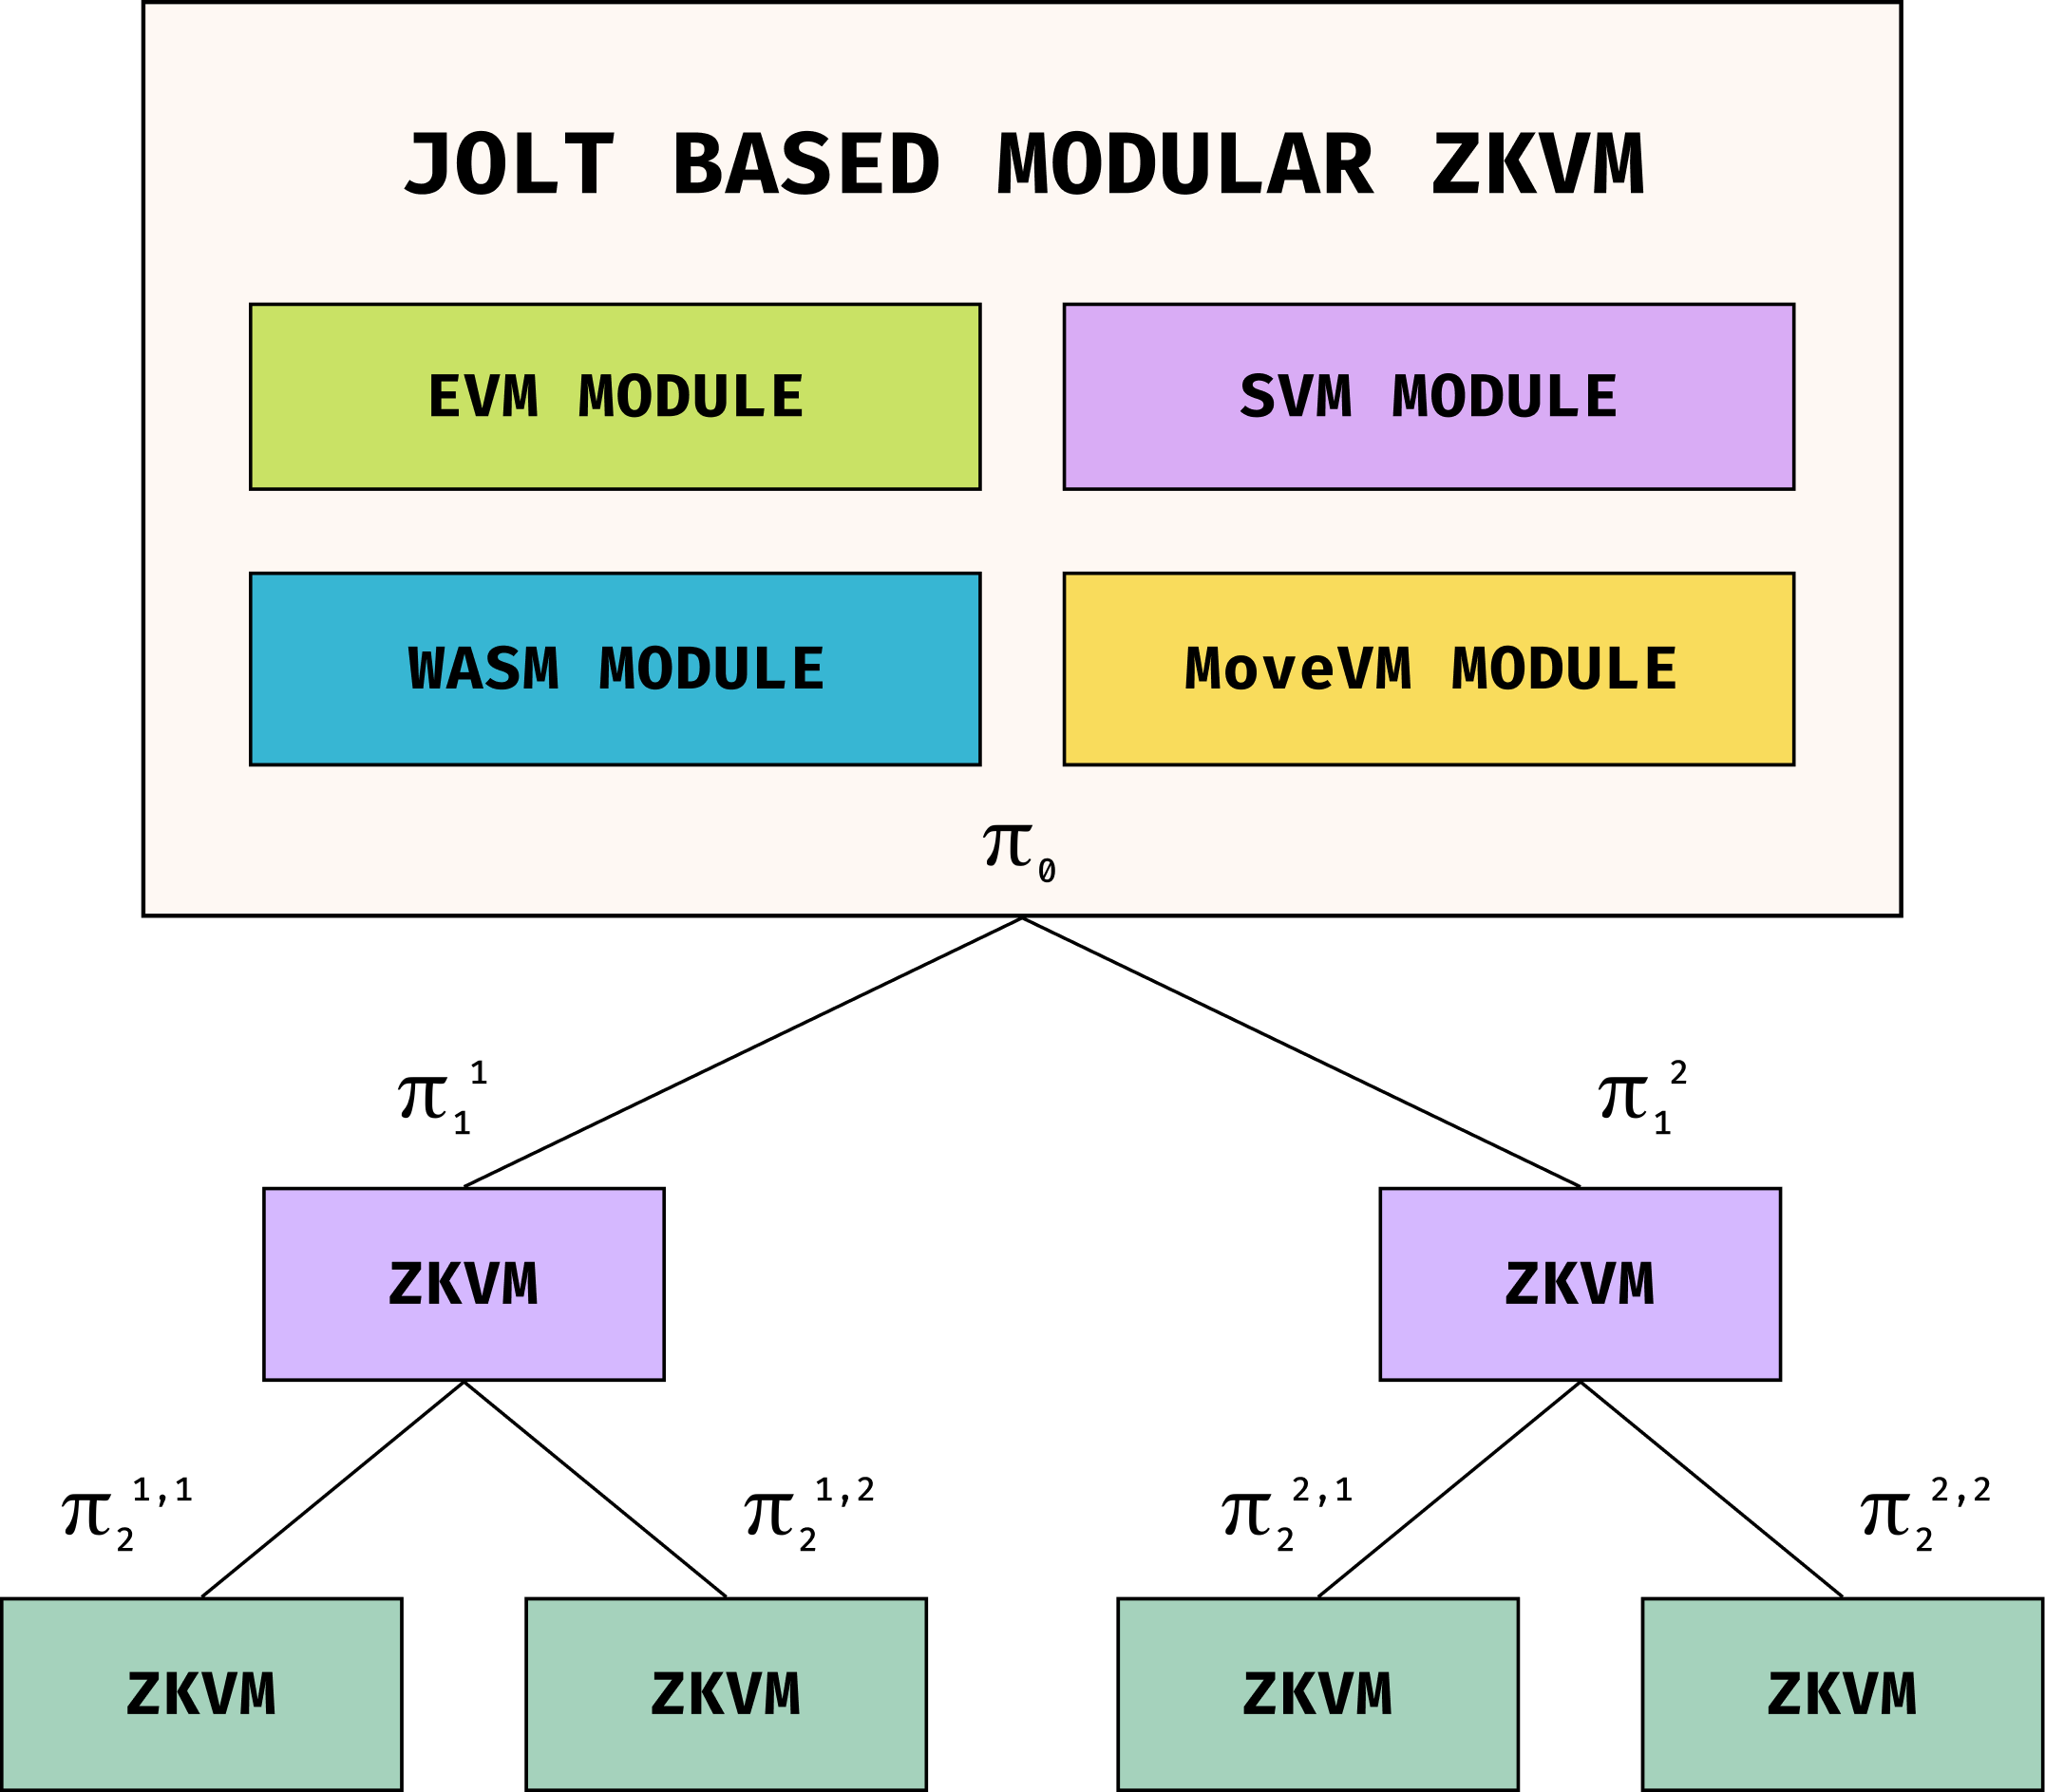
\includegraphics[width=0.7\linewidth]{figure/prover.png}
    \caption{Prover Network}
    \label{fig:prover}
\end{figure}

\subsubsection{Jolt zkVM}
The paper~\cite{jolt} introduces a novel approach to building zero-knowledge virtual machines (zkVMs) by leveraging a technique called Jolt. This method focuses on transforming program execution into a series of lookups into a predetermined, extensive lookup table, thereby enhancing efficiency and auditability in zkVMs. 

\begin{itemize}
    \item Lookup Singularity Vision: Jolt realizes the "lookup singularity" concept, aiming to design circuits that primarily perform lookups into a massive, predetermined table. This table, dependent solely on the instruction set architecture (ISA), is structured to avoid costs that scale linearly with its size, despite its theoretical enormity (e.g., size exceeding $2^128$). 

    \item Lasso Lookup Argument: To validate the lookups efficiently, Jolt employs a new lookup argument called Lasso, detailed in a companion work by Setty, Thaler, and Wahby. Lasso enables efficient proofs of correct execution by performing multiple lookups into smaller subtables and combining the results, facilitating the handling of massive structured tables without incurring prohibitive costs. 

    \item Application to RISC-V ISA: The paper demonstrates the application of Jolt to the RISC-V ISA, a widely adopted open standard. For 64-bit data types, the dominant cost for the Jolt prover is cryptographically committing to approximately six 256-bit field elements per RISC-V CPU step. This performance is favorable compared to prior zkVM providers, even those focused on simpler VMs. 

    \item Performance and Auditability Benefits: Jolt offers significant performance improvements and enhanced auditability over previous zkVMs. By reducing complex computations to structured table lookups, it simplifies the verification process and reduces the computational burden on the prover, leading to more efficient and transparent zkVM implementations. 

\end{itemize}


\subsubsection{Distributed Deployment of Jolt zkVM}  

Deploying the Jolt zkVM in a distributed form brings several advantages by leveraging a network of provers to parallelize computation and enhance scalability.  Distributes computation of zk proofs across multiple nodes, significantly reducing the time required for proof generation.  Increases resilience by ensuring that proof generation can continue even if some nodes in the network fail. Dynamically allocates workloads across nodes, ensuring efficient resource utilization. By deploying nodes geographically closer to the data sources or target blockchains, latency is minimized, and overall throughput is enhanced.  

The modular architecture of the Jolt zkVM is the cornerstone of efficient and isolated state management across multiple blockchains. By integrating specialized virtual machine modules, such as the EVM Module, SVM Module, MoveVM Module, and WASM Module, the zkVM can simultaneously maintain the states of various chains in a unified, yet independent manner, ensuring both interoperability and operational isolation. The EVM Module is designed to handle Ethereum-compatible chains, providing robust support for Solidity-based smart contracts and facilitating seamless state transitions within the Ethereum ecosystem. The SVM Module caters to Solana-compatible chains, leveraging Solana's high-performance architecture to enable rapid transaction processing and execution. The MoveVM Module enables compatibility with Move-based blockchains, such as Aptos and Sui, by using Move's resource-oriented programming model to enhance security, parallel execution, and asset integrity. The WASM Module supports chains based on WebAssembly (WASM), offering developers the flexibility to build and run applications in diverse programming languages such as Rust, C++, and more. 


This modularity not only enhances the zkVM's ability to manage cross-chain interactions efficiently but also provides a scalable framework for supporting an expanding ecosystem of blockchains with varying technical requirements. The combination of distributed deployment and modularity in the Jolt zkVM sets a new standard for zkVMs, providing unparalleled scalability, flexibility, and cross-chain capabilities to power the next generation of blockchain applications.
\subsection{Omni Rollup}

The Omni Rollup is a robust framework designed to facilitate cross-chain transactions across multiple Layer 1 (L1) blockchains within the Omnichain ecosystem. It deploys smart contracts on L1 chains that support them, managing transaction validation, state updates, and communication with the rollup. For L1 chains that do not support smart contracts, Omni Rollup uses direct addresses (vaults) to handle asset custody and processing. Execution within the rollup can be configured in two ways: a shared executor maintaining isolated states for each supported chain, ensuring resource optimization and centralized logic, or separate executors for each chain, which provide high isolation and allow chain-specific customizations.  

At the core of its operation is the Omni Sequencer, a shared transaction coordinator responsible for organizing and ordering transactions. The sequencer collects transactions from various mempools and solvers, bundles them into batches, and determines a global order. A commitment for this order is created by hashing the ordered list of transaction bundles, producing a cryptographic digest that is published on a Data Availability (DA) layer. This commitment ensures that all participants can verify the integrity of the transaction order without accessing all transaction data. Each bundled transaction follows a specific format, comprising the source and destination chain IDs, the transaction payload, a timestamp, and a unique nonce to prevent replay attacks.  

Once the order is committed, the Omni Sequencer distributes the bundled transactions to the respective rollups for block creation. Each rollup verifies the transaction order against the commitment on the DA layer and uses the Prover network to validate state transitions. The Prover Network generates zero-knowledge (zk) proofs to confirm state correctness and prevent fraudulent updates. The rollup then updates the state of its respective chain and sends the updated state along with the zk proof to the L1 chain for final inclusion in its block. For non-contract-based chains, the proof will be sent to a client for verification. 
\begin{figure}[h!]
    \centering
    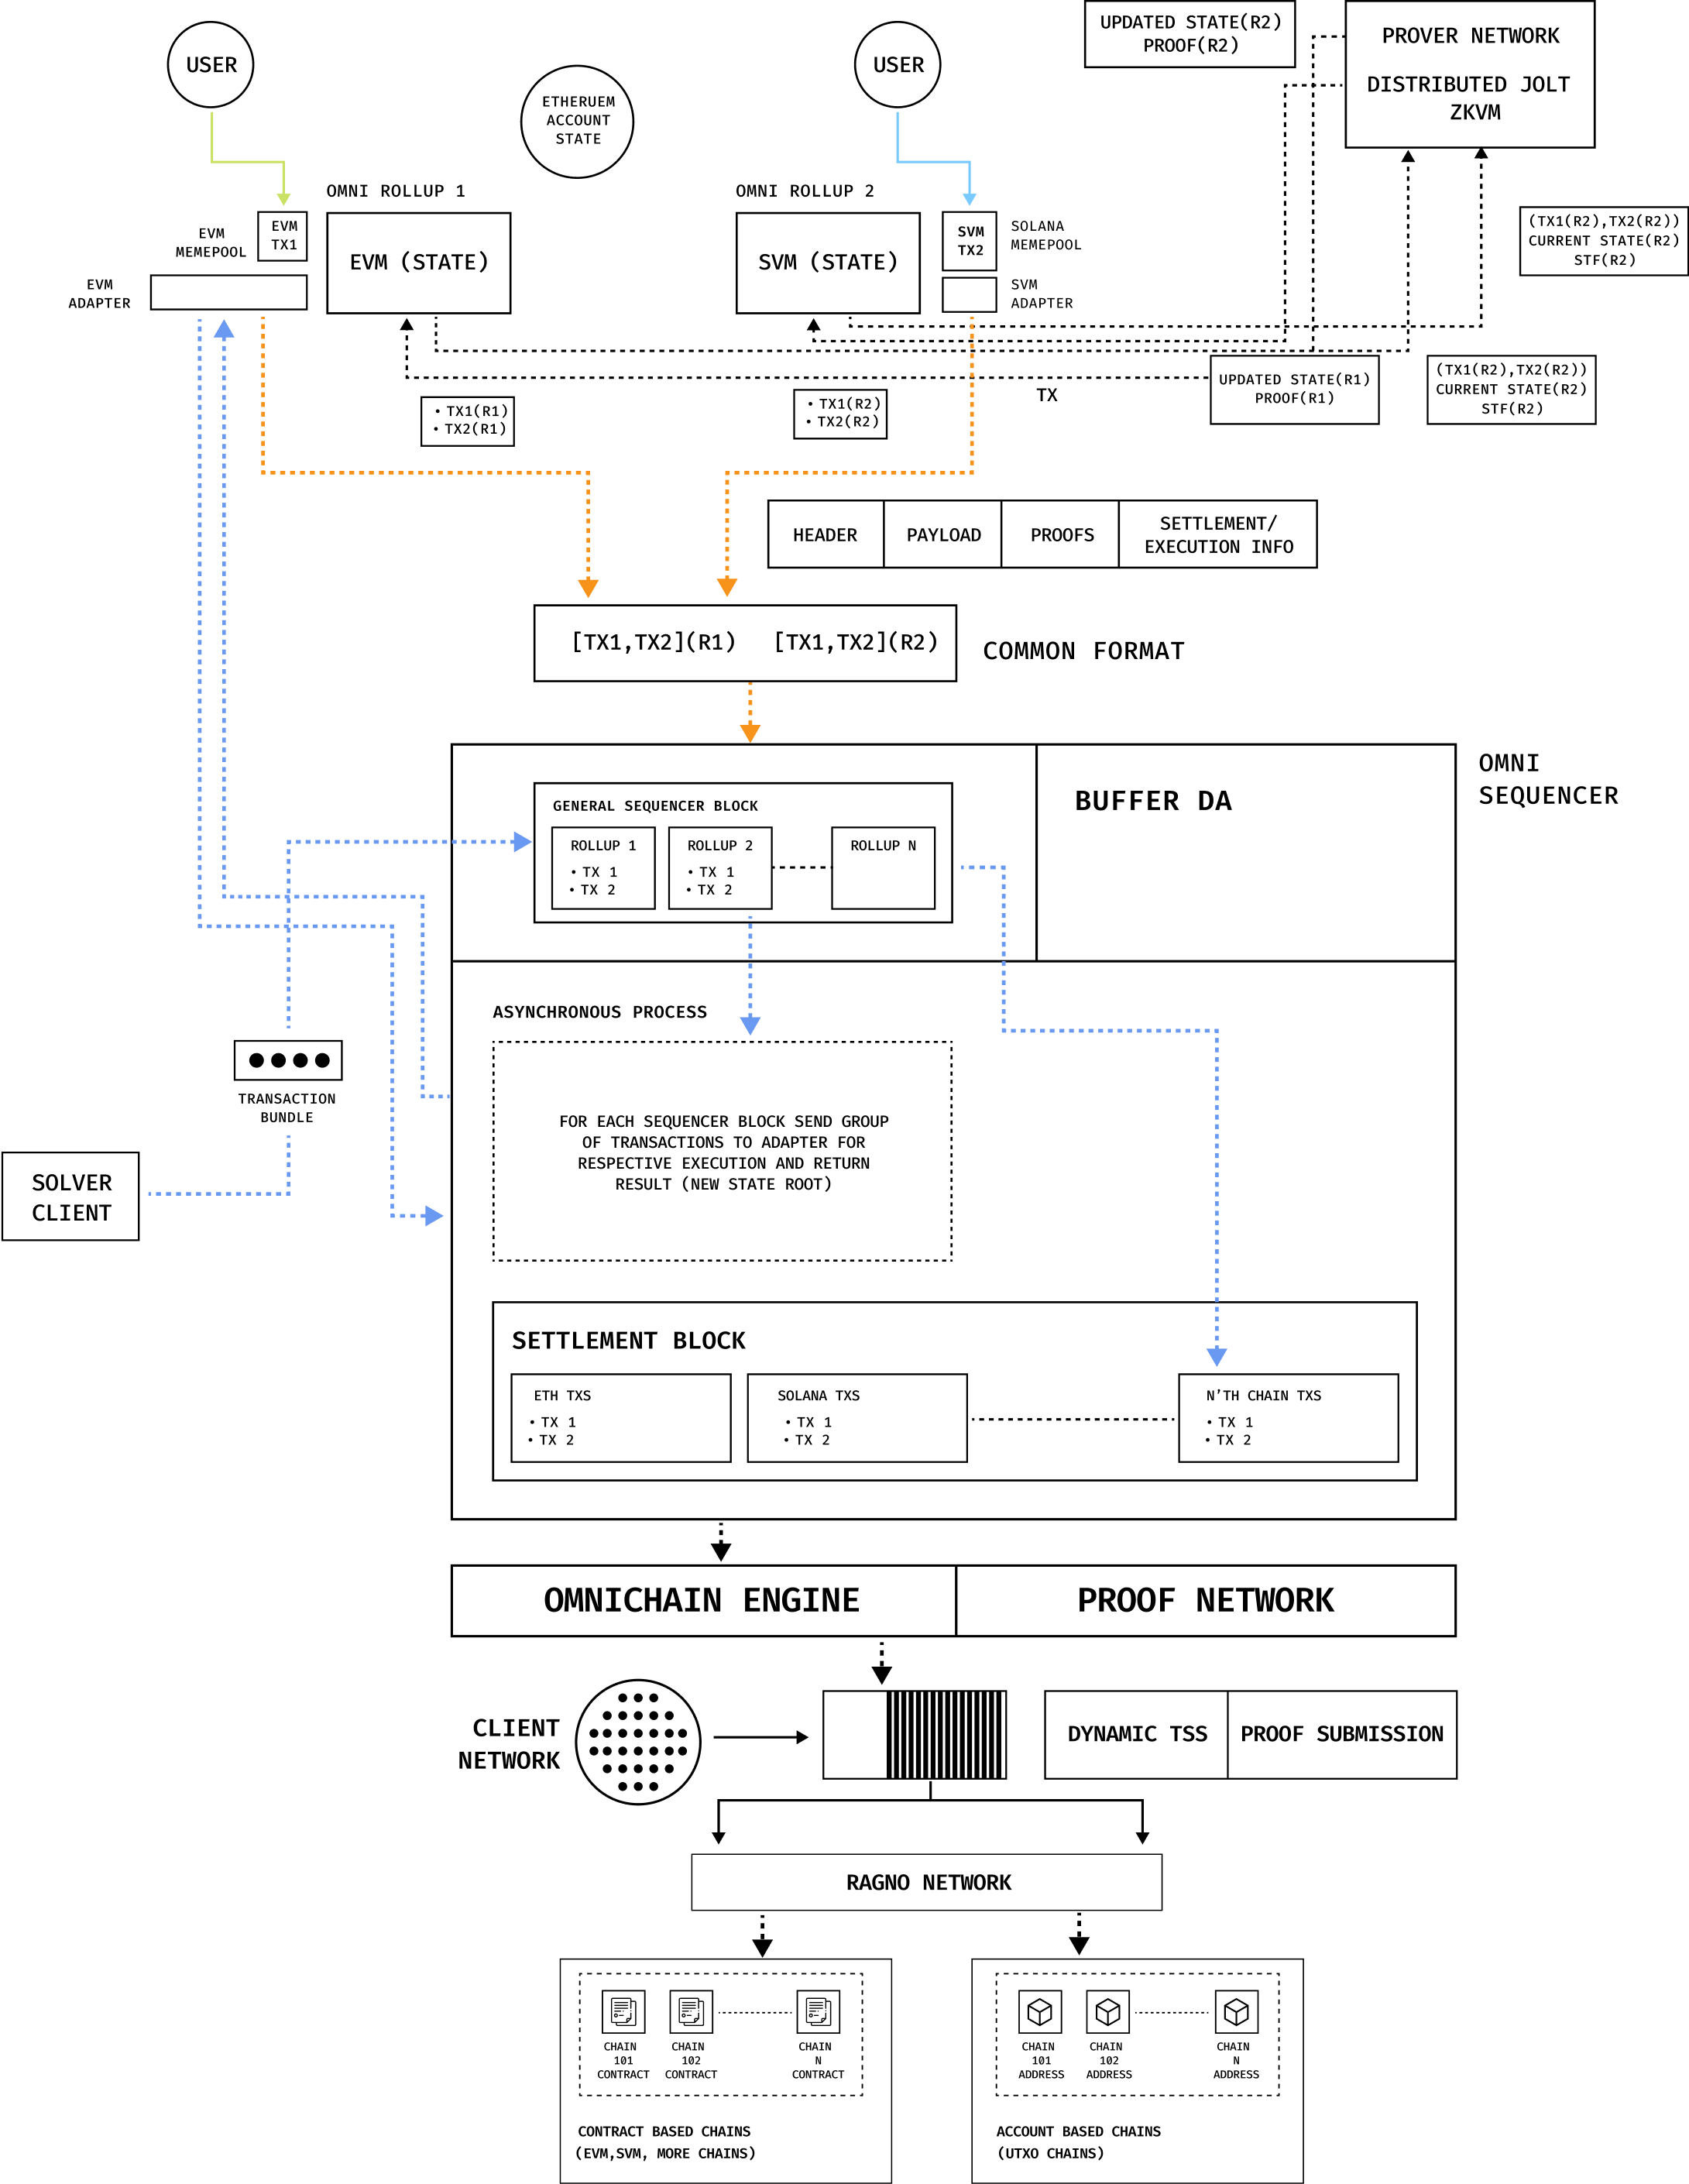
\includegraphics[width=0.99\linewidth]{figure/rollup.png}
    \caption{Omni Rollup Illustration}
    \label{fig:rollup}
\end{figure}
This architecture ensures scalability by efficiently bundling and ordering transactions, security through zk proofs and commitments, and interoperability by supporting both contract-enabled and other chains. The flexible executor configurations enable adaptation to diverse performance and isolation needs, making the Omni Rollup a critical component of the Omnichain web for seamless cross-chain transaction processing.



\subsubsection{Linera Microchains}

Linera~\cite{linera} introduces an innovative blockchain architecture centered around microchains, which are lightweight chains operating in parallel within a shared set of validators. This design separates the roles of block proposal and validation, often delegating block production to users themselves. Such an approach allows for an unlimited number of microchains to run concurrently, ensuring low transaction fees, rapid finality, and direct user access to on-chain data.

Linera’s core innovation lies in its microchain model, which is designed to scale Web3 applications predictably while taking advantage of modern cloud infrastructure. Key aspects include:
\begin{itemize}
    \item Elastic Validators: Validators function as scalable Web2-like services that validate and execute transactions across many microchains in parallel.
    
    \item User-Owned Microchains: Users own and maintain their own microchains, separating block production from validation.

    \item Integrated Multi-Chain Approach: Each validator manages all microchains, enabling asynchronous cross-chain messaging and parallel execution.

    \item Cross-Chain Messaging: Validators manage internal network communication between microchains to enable interoperability.

    \item Low-Latency Block Submission: Users submit blocks directly to validators without relying on a mempool, ensuring fast processing.

    \item Validator Independence: Validators do not interact with each other except for public chains owned by Linera’s infrastructure. Synchronization is handled by chain owners, and inactive chains impose no computational cost beyond storage.
\end{itemize}

Every validator maintains a map containing the states of all microchains, indexed by their identifiers. Clients track the state of only a subset of relevant chains, acting as full nodes only for those chains. This ensures efficient state management and reduces the computational burden on users.
Linera supports a theoretically unlimited number of microchains, allowing Web3 applications to maintain predictable performance at scale.

In conclusion,Linera’s microchain-based architecture provides a scalable, efficient, and user-friendly solution to traditional blockchain limitations. By decoupling block production from validation and leveraging elastic validators, Linera achieves the performance necessary for large-scale decentralized applications while maintaining decentralization and efficiency.



\subsubsection{Different Types of Rollups}
We are considering all different possibilities for cross-chain rollups. Along with omni-rollup, we are going to support existing and any private rollup as well with our cross-chain ecosystem. 

\begin{itemize}
    \item \textbf{Omni Rollup with Shared Executor}
    
    This architecture leverages a shared executor to oversee the states of all supported chains within a unified framework. The shared executor ensures efficient processing of cross-chain transactions while maintaining isolated state management for each chain, preventing conflicts, and preserving chain-specific integrity. This design simplifies interchain communication, but it necessitates robust mechanisms to mitigate state interference and establish trust in the shared execution layer. It is particularly well-suited for streamlined cross-chain dApps that benefit from a unified transaction coordinator.

 \begin{figure}[h!]
    \centering
    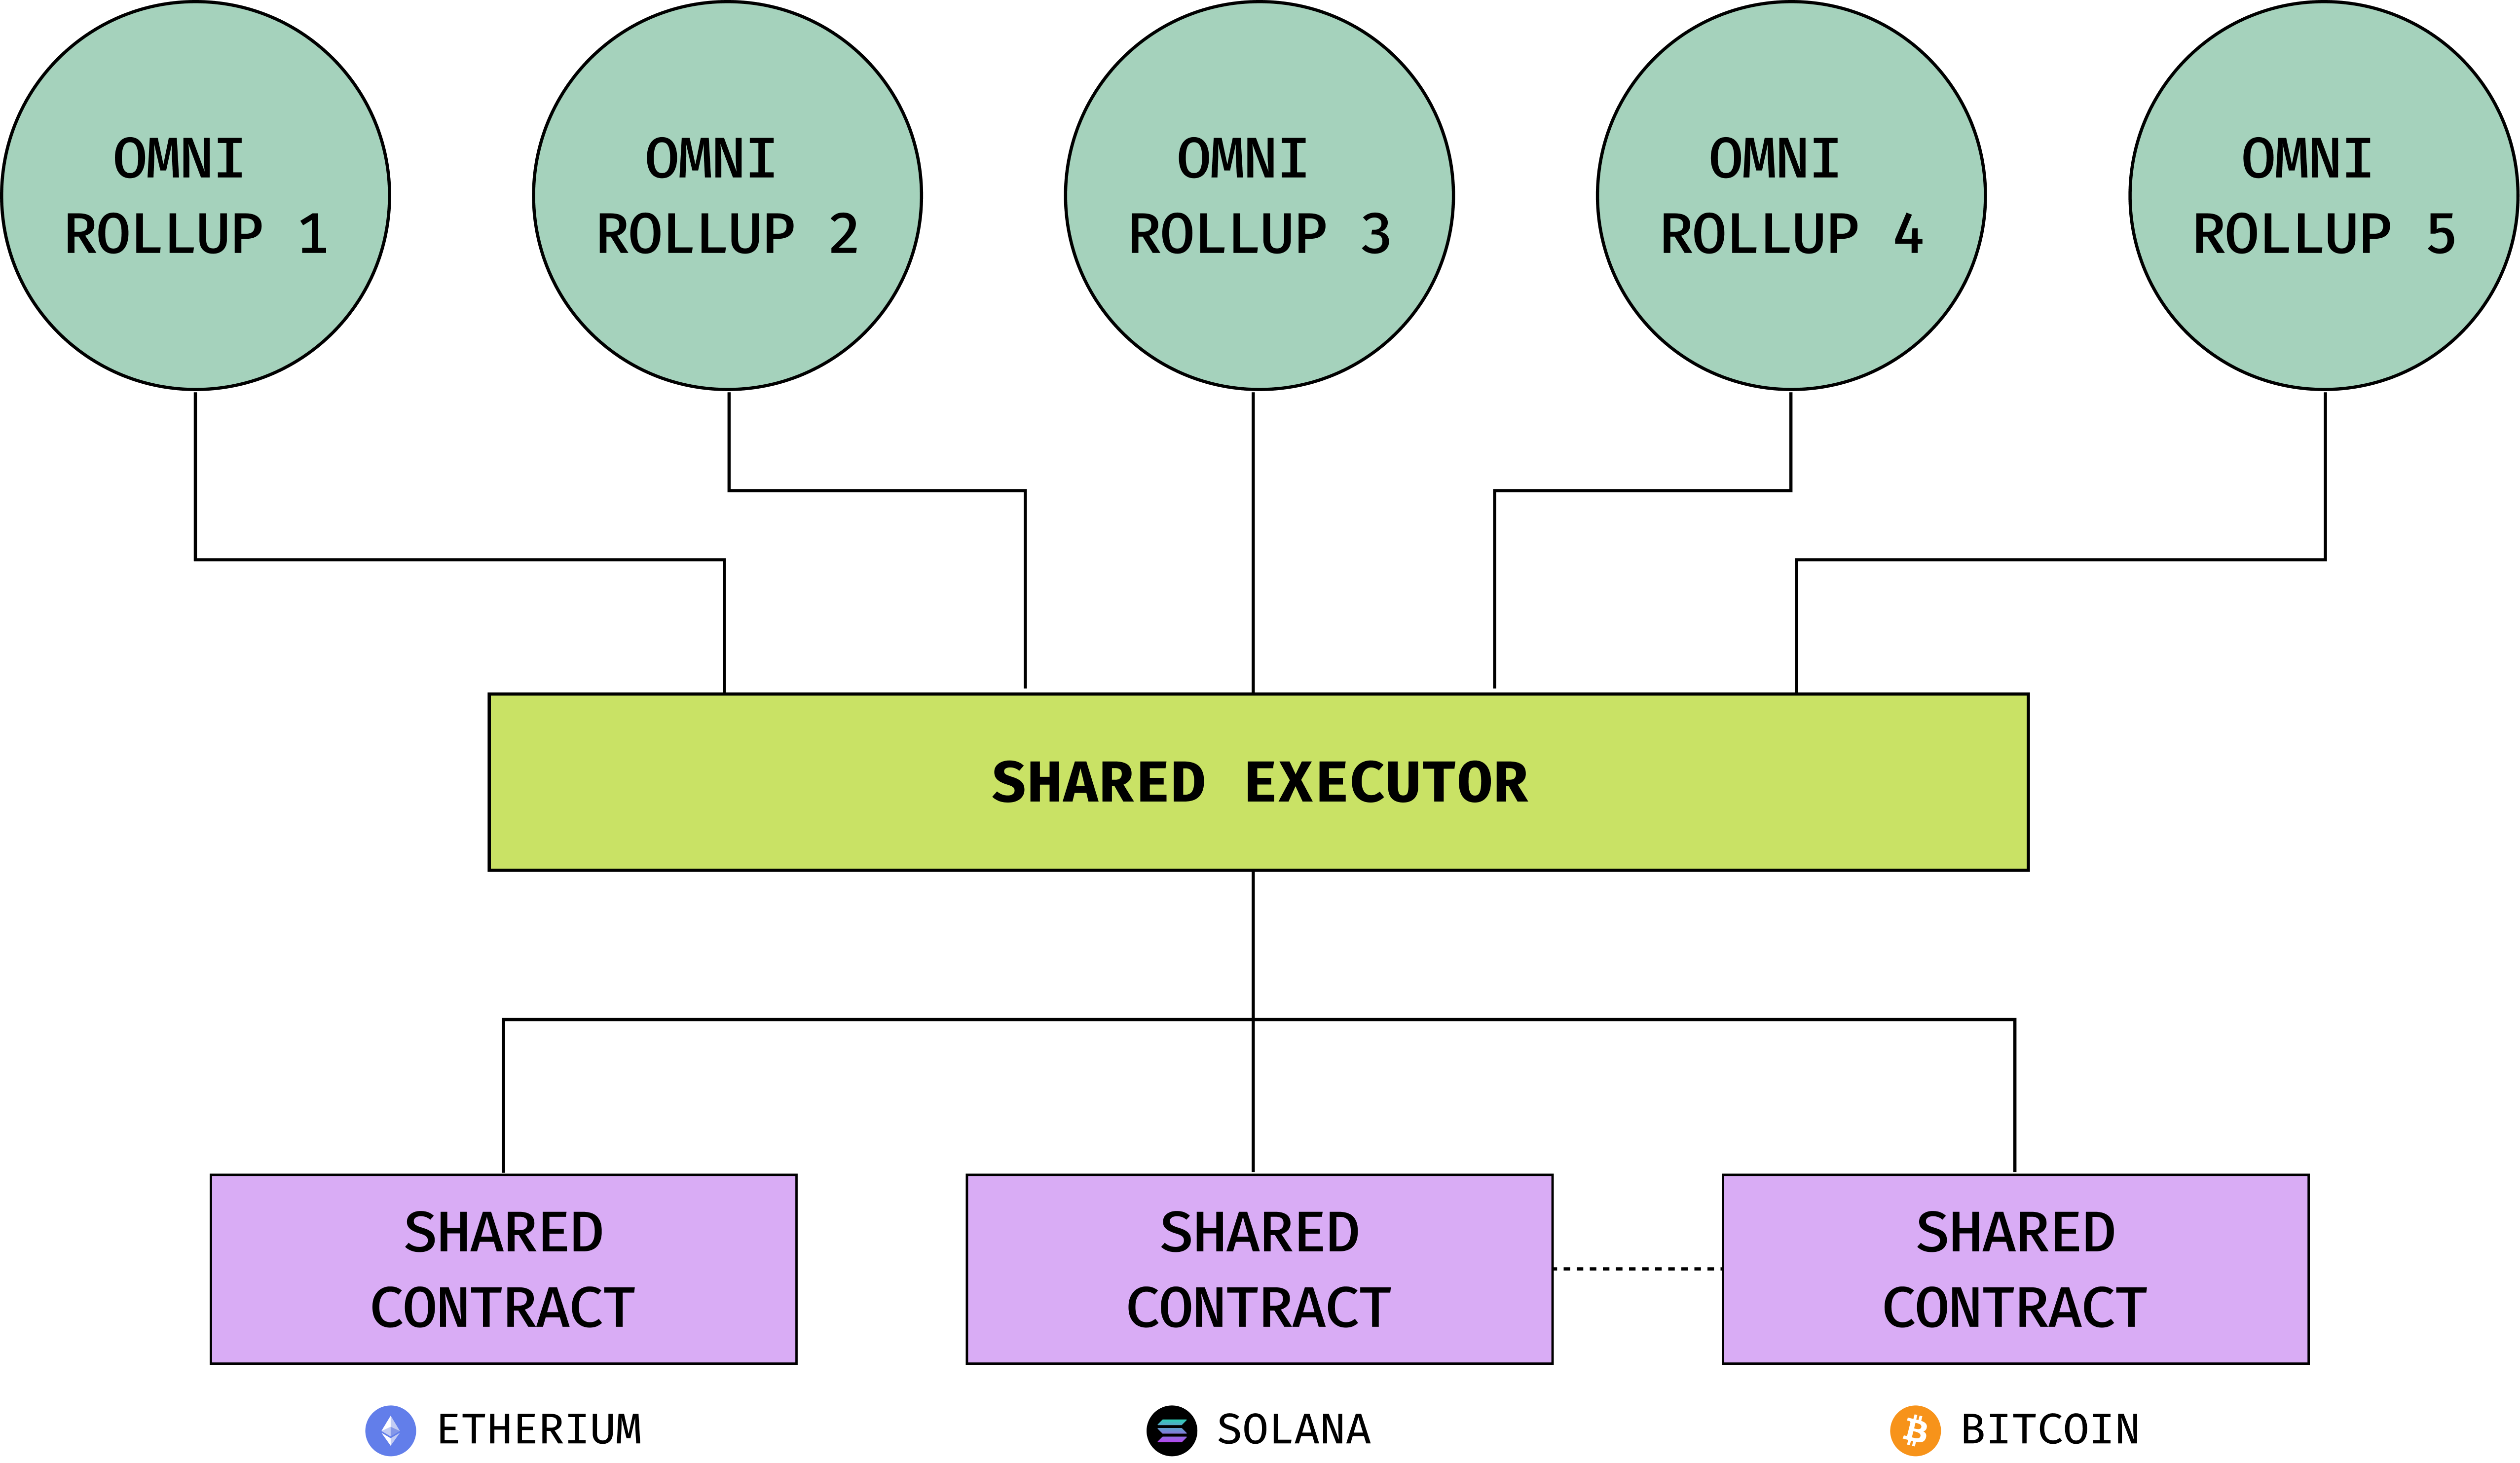
\includegraphics[width=0.9\linewidth]{figure/shared.png}
    \caption{Omni Rollup With Shared Executor}
    \label{fig:shared_rollup}
\end{figure}


    \item \textbf{Omni Rollup with Dedicated Executors for Each Chain}  

    In this setup, each supported chain operates with its own dedicated execution layer, ensuring autonomous state management while remaining part of the broader omnichain framework. This modular architecture improves resilience and scalability by isolating execution responsibilities per chain. However, advanced protocols are required for interoperability to ensure seamless cross-chain consistency and coordination. This approach is ideal for applications that require independent chain control in conjunction with flexible and efficient cross-chain interactions.
 \begin{figure}[h!]
    \centering
    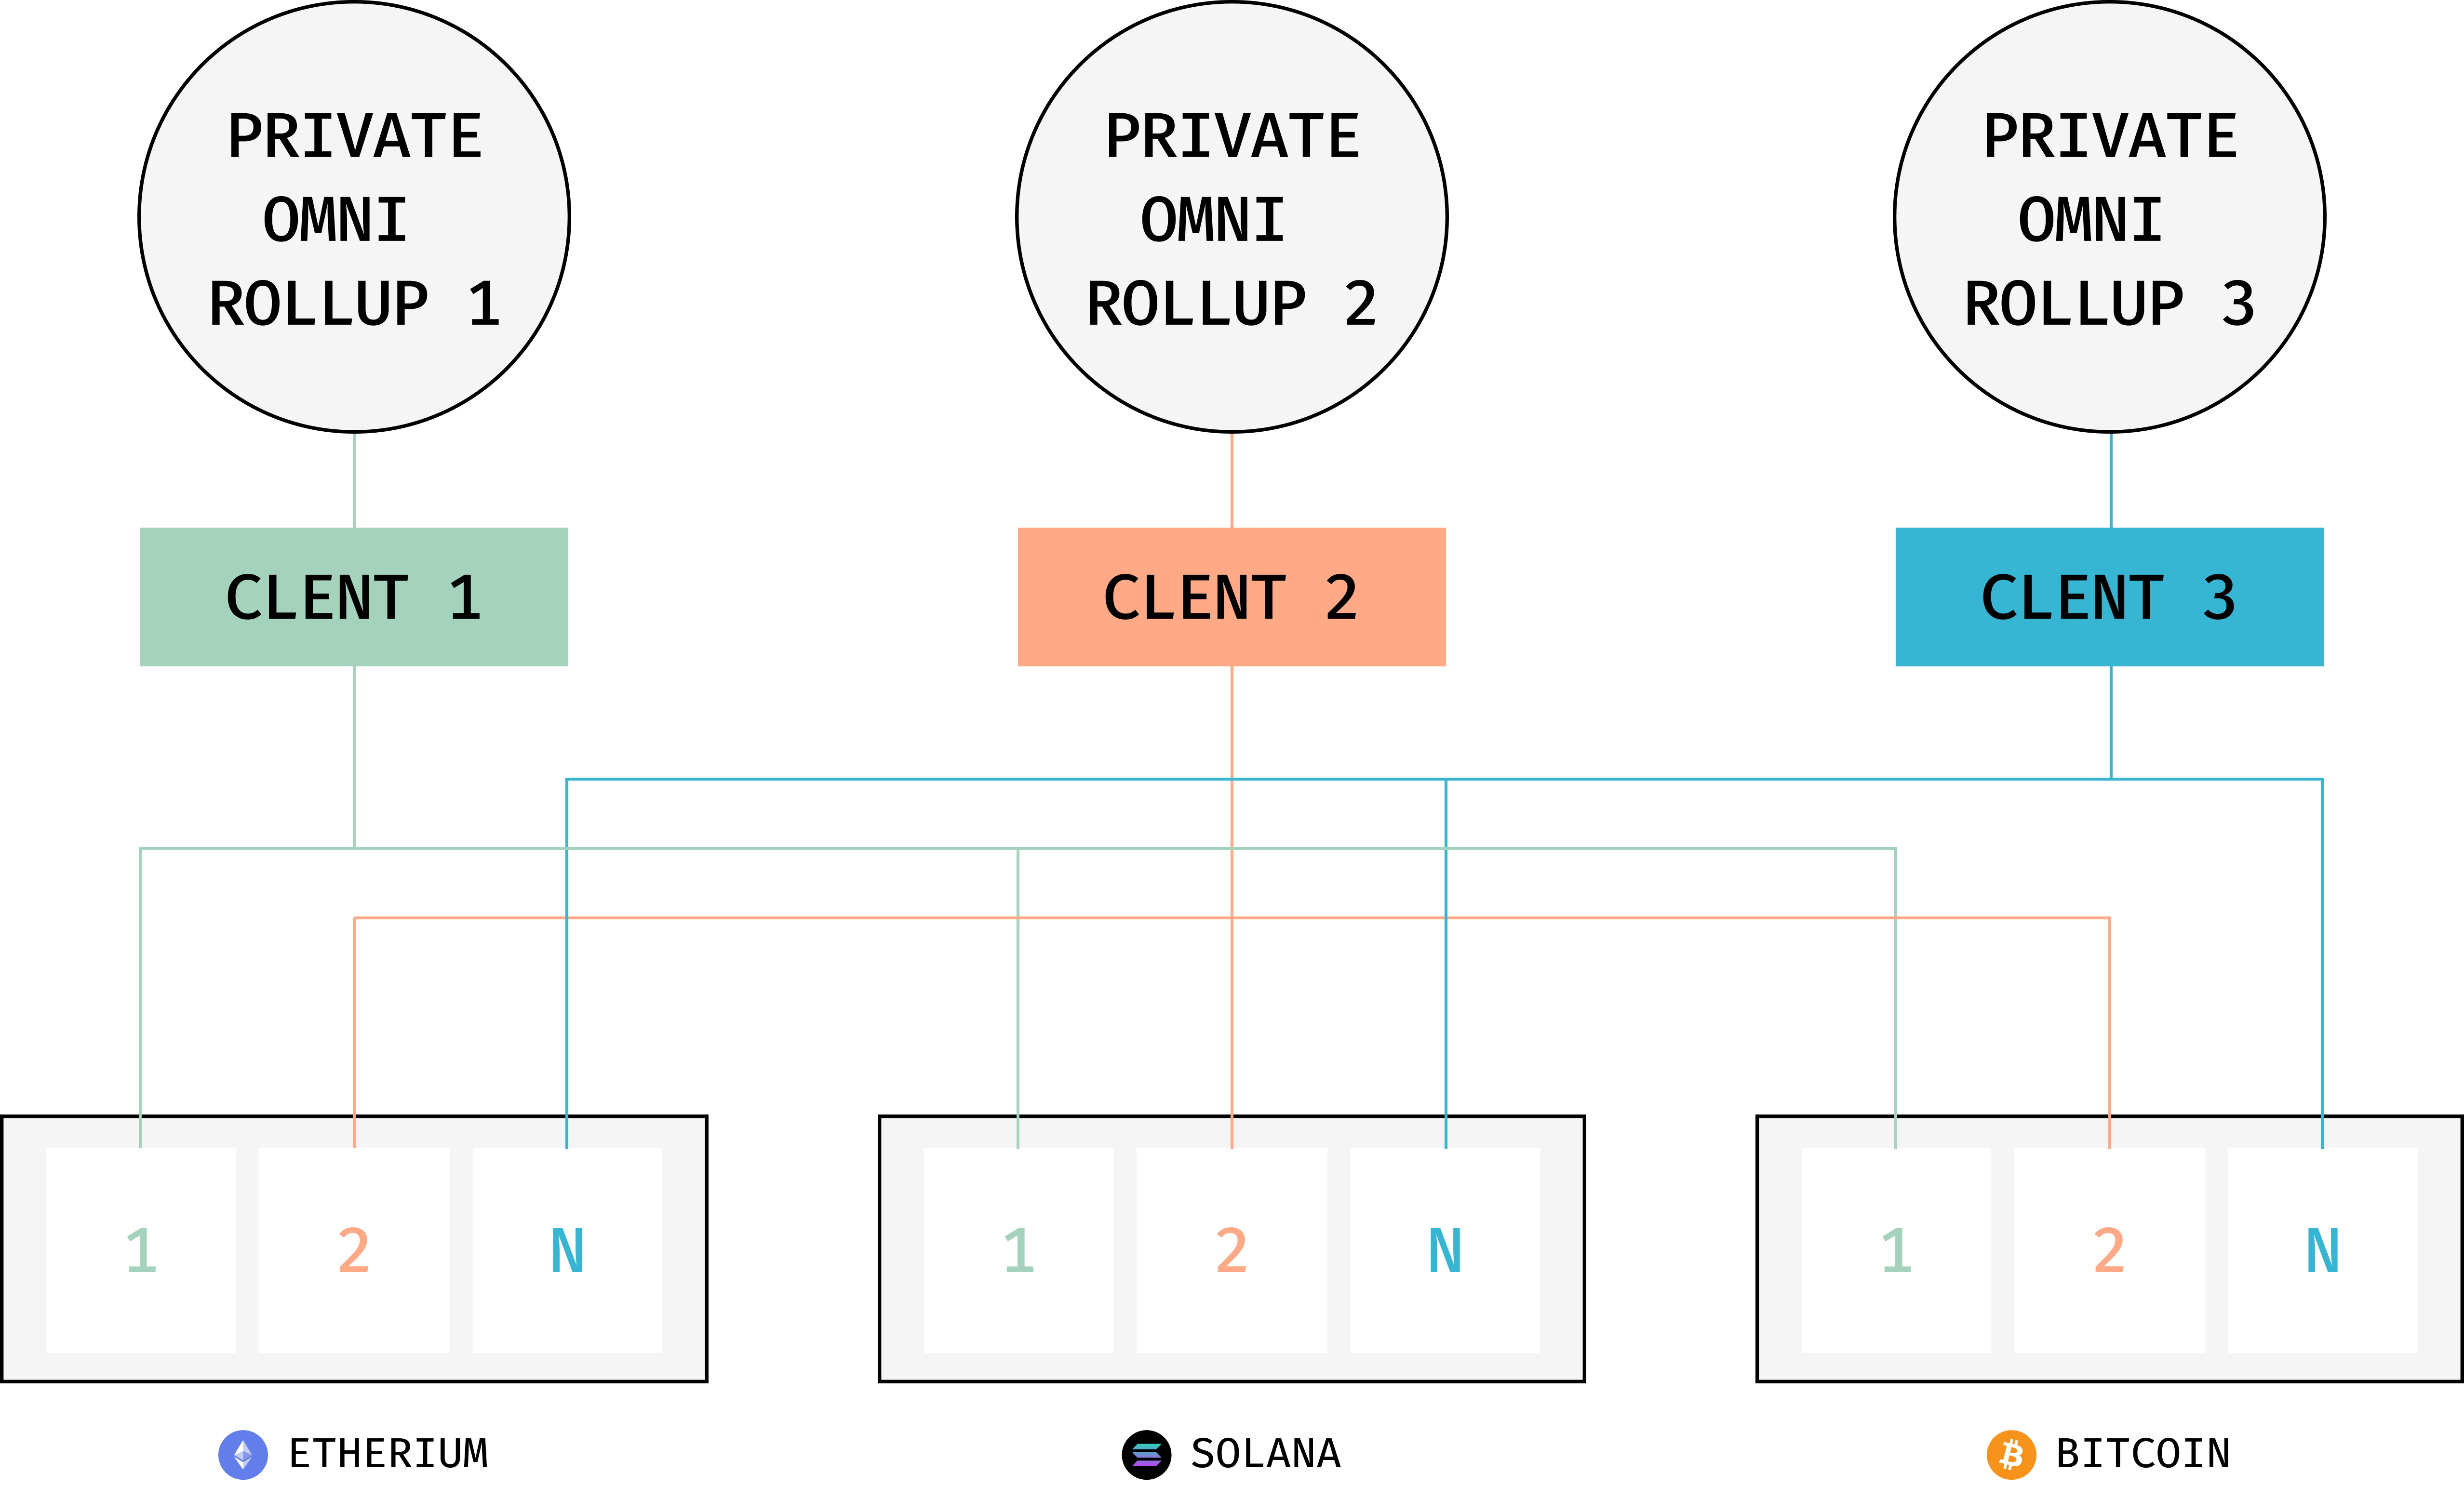
\includegraphics[width=0.9\linewidth]{figure/separate.png}
    \caption{Omni Rollup With Dedicated Executor}
    \label{fig:separate_rollup}
\end{figure}

    \item \textbf{Adapter-Enabled Omni Rollup}  

    This approach builds on existing roll-up infrastructures, transforming them into omni-chain runs through the use of adapters or clients. These adapters facilitate seamless cross-chain communication and functionality without requiring significant modifications to the existing rollup architecture. This method provides a low-barrier entry for projects to integrate into the omnichain ecosystem while preserving their original operational framework. It enables a smooth transition of legacy roll-ups into the omnichain paradigm with minimal disruption.

    \item \textbf{Private Omni Rollup for Enterprise Use}  

    A private omnichain rollup is tailored for enterprise entities to facilitate secure and controlled cross-chain operations. These rollups are maintained by the enterprise itself, with full autonomy over the network execution, consensus, and state management. Designed for privacy and control, they are ideal for corporate applications such as cross-chain payments, supply chain tracking, and private inter-organization workflows. Enterprise solutions requiring controlled, private, and efficient cross-chain infrastructure.  
\end{itemize}

In our omnichain architecture, we are planning to launch a range of omnichain roll-ups, with the potential to scale to tens or even hundreds of thousands. To support this scalability, it is essential that each rollup have secure and decentralized access to its state. This ensures efficient transaction validation and integrity across the entire ecosystem. To achieve this, we collaborated with Linera Microchains. These microchains offer a robust solution by allowing each one to operate independently with its own isolated state. This modularity guarantees that the Omnichain Engine and Sequencer can securely access and validate transactions across all roll-ups, without compromising decentralization or security.

For simpler roll-ups, we will run a Linera node connected to the Ragno Network, providing seamless and straightforward state management. However, for more complex roll-ups with higher liquidity and intricate structures, we will deploy dedicated nodes for each L2/roll-up. This ensures both strong connectivity and thorough verification of transactions. Each microchain will integrate omnichain logic, acting as an intermediary to forward transactions to the sequencer or Hermes, depending on the destination. This setup not only enhances the flexibility and scalability of our solution but also ensures that validation and verification remain fully decentralized, with dedicated validators for each roll-up and microchain.

\subsubsection{Omni Sequencer: The Core of the Omnichain Stack}

The Omni Sequencer is the foundational component of the Omnichain Stack, acting as the central coordination layer for Omni Rollups. It ensures seamless cross-rollup execution, atomic transaction processing, and efficient bundling of transactions across multiple rollup environments. By integrating with both converted L2 rollups (e.g., Optimism, Arbitrum, zkSync, and Movement Labs rollups) and native Omni-rollups, the Omni Sequencer transforms them into fully interoperable Omnichain ecosystems.

 \begin{figure}[h!]
    \centering
    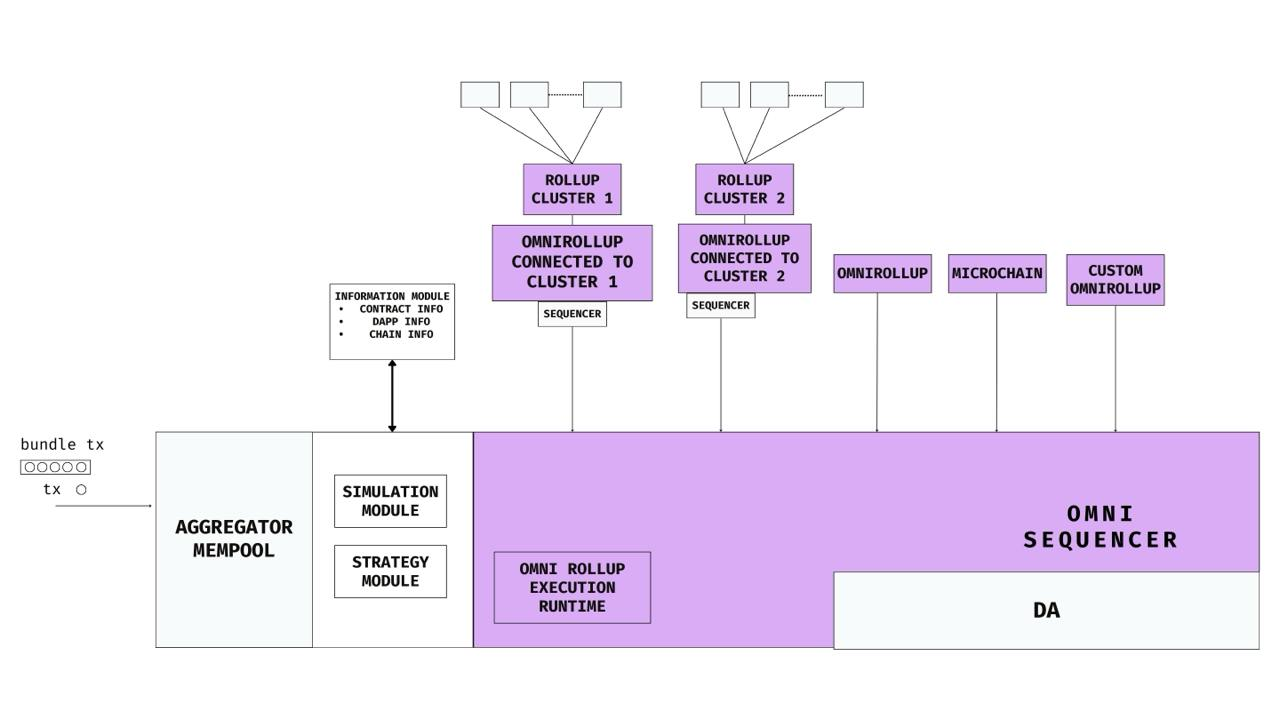
\includegraphics[width=0.99\linewidth]{figure/omnisequencer.jpg}
    \caption{Omnisequencer Overview}
    \label{fig:separate_rollup}
\end{figure}

\textbf{Key Functional Modules of the Omni Sequencer}

\begin{itemize}
    \item[1.] Simulation Module: Ensures atomic execution of transactions across multiple rollups. Simulates transactions before execution to guarantee validity and prevent failures. Reduces transaction reverts by pre-validating state transitions before final submission.

    \item[2.] Strategy Module: Manages transaction ordering and execution logic for cross-rollup transaction bundles. Determines execution priorities based on efficiency, MEV considerations, and state dependencies. Optimizes for low-latency execution and economic efficiency.

    \item[3.] Omni Rollup Execution Runtime: Queries and simulates transaction execution across multiple chains. Facilitates state-aware cross-rollup communication by ensuring each transaction’s dependencies are met. Enhances developer experience by abstracting cross-chain execution complexity.

    \item[4.] Aggregate Mempool: Collects both bundled and individual transactions before execution. Optimizes block space usage by prioritizing transactions based on gas efficiency and finality requirements. Reduces fragmentation in cross-rollup transaction processing.
    
    \item[5.] Data Availability Integration: The Omni Sequencer integrates with multiple DA layers (Data Availability layers) while also maintaining its own Omnichain Data Availability Layer. Enhances data integrity, accessibility, and redundancy across connected rollups. Ensures seamless rollup-to-rollup communication without external dependencies on third-party DA layers.

\end{itemize}
By anchoring the Omnichain Stack, the Omni Sequencer enables true interoperability across rollups. It bridges fragmented L2 ecosystems into a unified execution environment, ensuring that transactions across different chains execute atomically, efficiently, and securely. With its integration of cross-rollup mempools, simulation layers, and DA enhancements, the Omni Sequencer is a game-changer in modular blockchain architecture.

\subsubsection{Transaction Flow and Execution}  
The transaction workflow within the Omni Rollup is a multistage process designed for efficiency, scalability, and cross-chain synchronization. Transactions can originate from various sources, including user submissions, application interactions, or solvers, and are directed to the Omni Sequencer via mempools or other submission mechanisms. Additionally, the sequencer can directly accept transactions initiated on Layer 1 (L1) blockchains through a crawler. The crawler captures and validates these L1 transactions, forwarding them to the Omnichain Engine for direct settlement on the originating L1 chain, bypassing rollups when necessary.  

Once transactions are received, the sequencer organizes them based on predefined criteria such as the target blockchain, the type of operation, or the priority. Within each group, the sequencer determines an optimized execution order to maintain consistency and minimize resource overhead. The ordered transactions are compiled into bundles, with each bundle containing essential metadata, including source and destination chain IDs, timestamps, transaction payloads, and unique nonces to prevent replay attacks.  

To ensure transaction integrity, the Omni Sequencer uses a commitment mechanism. After compiling and ordering the bundles, it generates a cryptographic hash of the ordered transaction list, referred to as the commitment. This hash is published on the Data Availability (DA) Layer, ensuring transparency and allowing participants to validate the accuracy of the transaction order by comparing the commitment with the actual processing sequence during execution.  

The sequencer then distributes the bundled transactions to the appropriate rollups for execution. Each rollup begins by verifying the transaction order against the commitment published on the DA layer, ensuring alignment with the global sequence determined by the sequencer. Transactions are processed in accordance with this verified order, and the rollup computes state transitions for the respective blockchain or application.  

To guarantee security and integrity, the rollup uses zero-knowledge (zk) proofs generated by the Prover Network. These zk proofs validate the correctness of state transitions without exposing sensitive data, ensuring that the process is both tamperproof and privacy-preserving. For contract-enabled blockchains, rollups interact directly with smart contracts to manage state updates, validate proofs, and finalize transactions on the L1 chain. For blockchains without smart contract support, the rollup uses direct addresses, also known as vaults, as custodial points for assets and data. These vaults ensure that transactions and state updates are accurately reflected despite the lack of native contract capabilities.  

In both cases, rollups send the updated states and zk proofs to the respective L1 chains for inclusion in their blocks. This ensures that state changes are synchronized across the network, maintaining consistency across all connected chains. By supporting both direct L1 transactions and rollup-based processing, Omni Rollup establishes a robust, scalable, and trustless framework for cross-chain transactions, enhancing interoperability, and ensuring data integrity across diverse blockchain ecosystems.  

\subsubsection{Transaction Conflict Resolution}
The Omni Sequencer employs a robust mechanism to detect and resolve transaction conflicts, ensuring consistency and preventing double spending on multiple rollups. To achieve this, the sequencer maintains a global transaction pool, aggregating all incoming transactions, including those targeting different rollups. Before determining the execution order, the sequencer analyzes the input dependencies of each transaction (for example, the user's ETH balance). If multiple transactions reference the same input, a dependency conflict is detected.

In such cases, the sequencer assigns a global execution order to all transactions. Among conflicting transactions (e.g., double-spend attempts), only the first valid transaction in the sequence is included for execution, while subsequent conflicting transactions are marked as invalid or rejected outright. The ordered transactions, along with a cryptographic commitment to their order, are published on the Data Availability (DA) layer, ensuring transparency and verifiability. The sequencer then distributes the bundled transactions to their respective rollups for execution.

Each rollup verifies the transaction order against the published commitment. Transactions flagged as invalid or rejected by the sequencer are excluded during execution. This ensures that only valid transactions progress to state updates, maintaining the integrity and consistency of operations across all rollups in the Omnichain ecosystem.
\subsection{Builder Marketplace}
The Builder Marketplace is a next-generation ecosystem designed to streamline cross-chain communication for decentralized applications (dApps) by leveraging a network of modular solvers. These solvers integrate existing blockchain protocols across multiple chains, ensuring seamless interoperability and enhanced functionality for dApps. Our approach is unique in that we aggregate existing protocols from all blockchain networks and create modular representations of each dApp within our architecture. These dApp modules encapsulate all relevant information about a given application, enabling official teams to access, manage, and update their modules through a dedicated dashboard, similar to how APIs are managed and deployed on platforms like Postman today.

\begin{figure}[h]
    \centering
    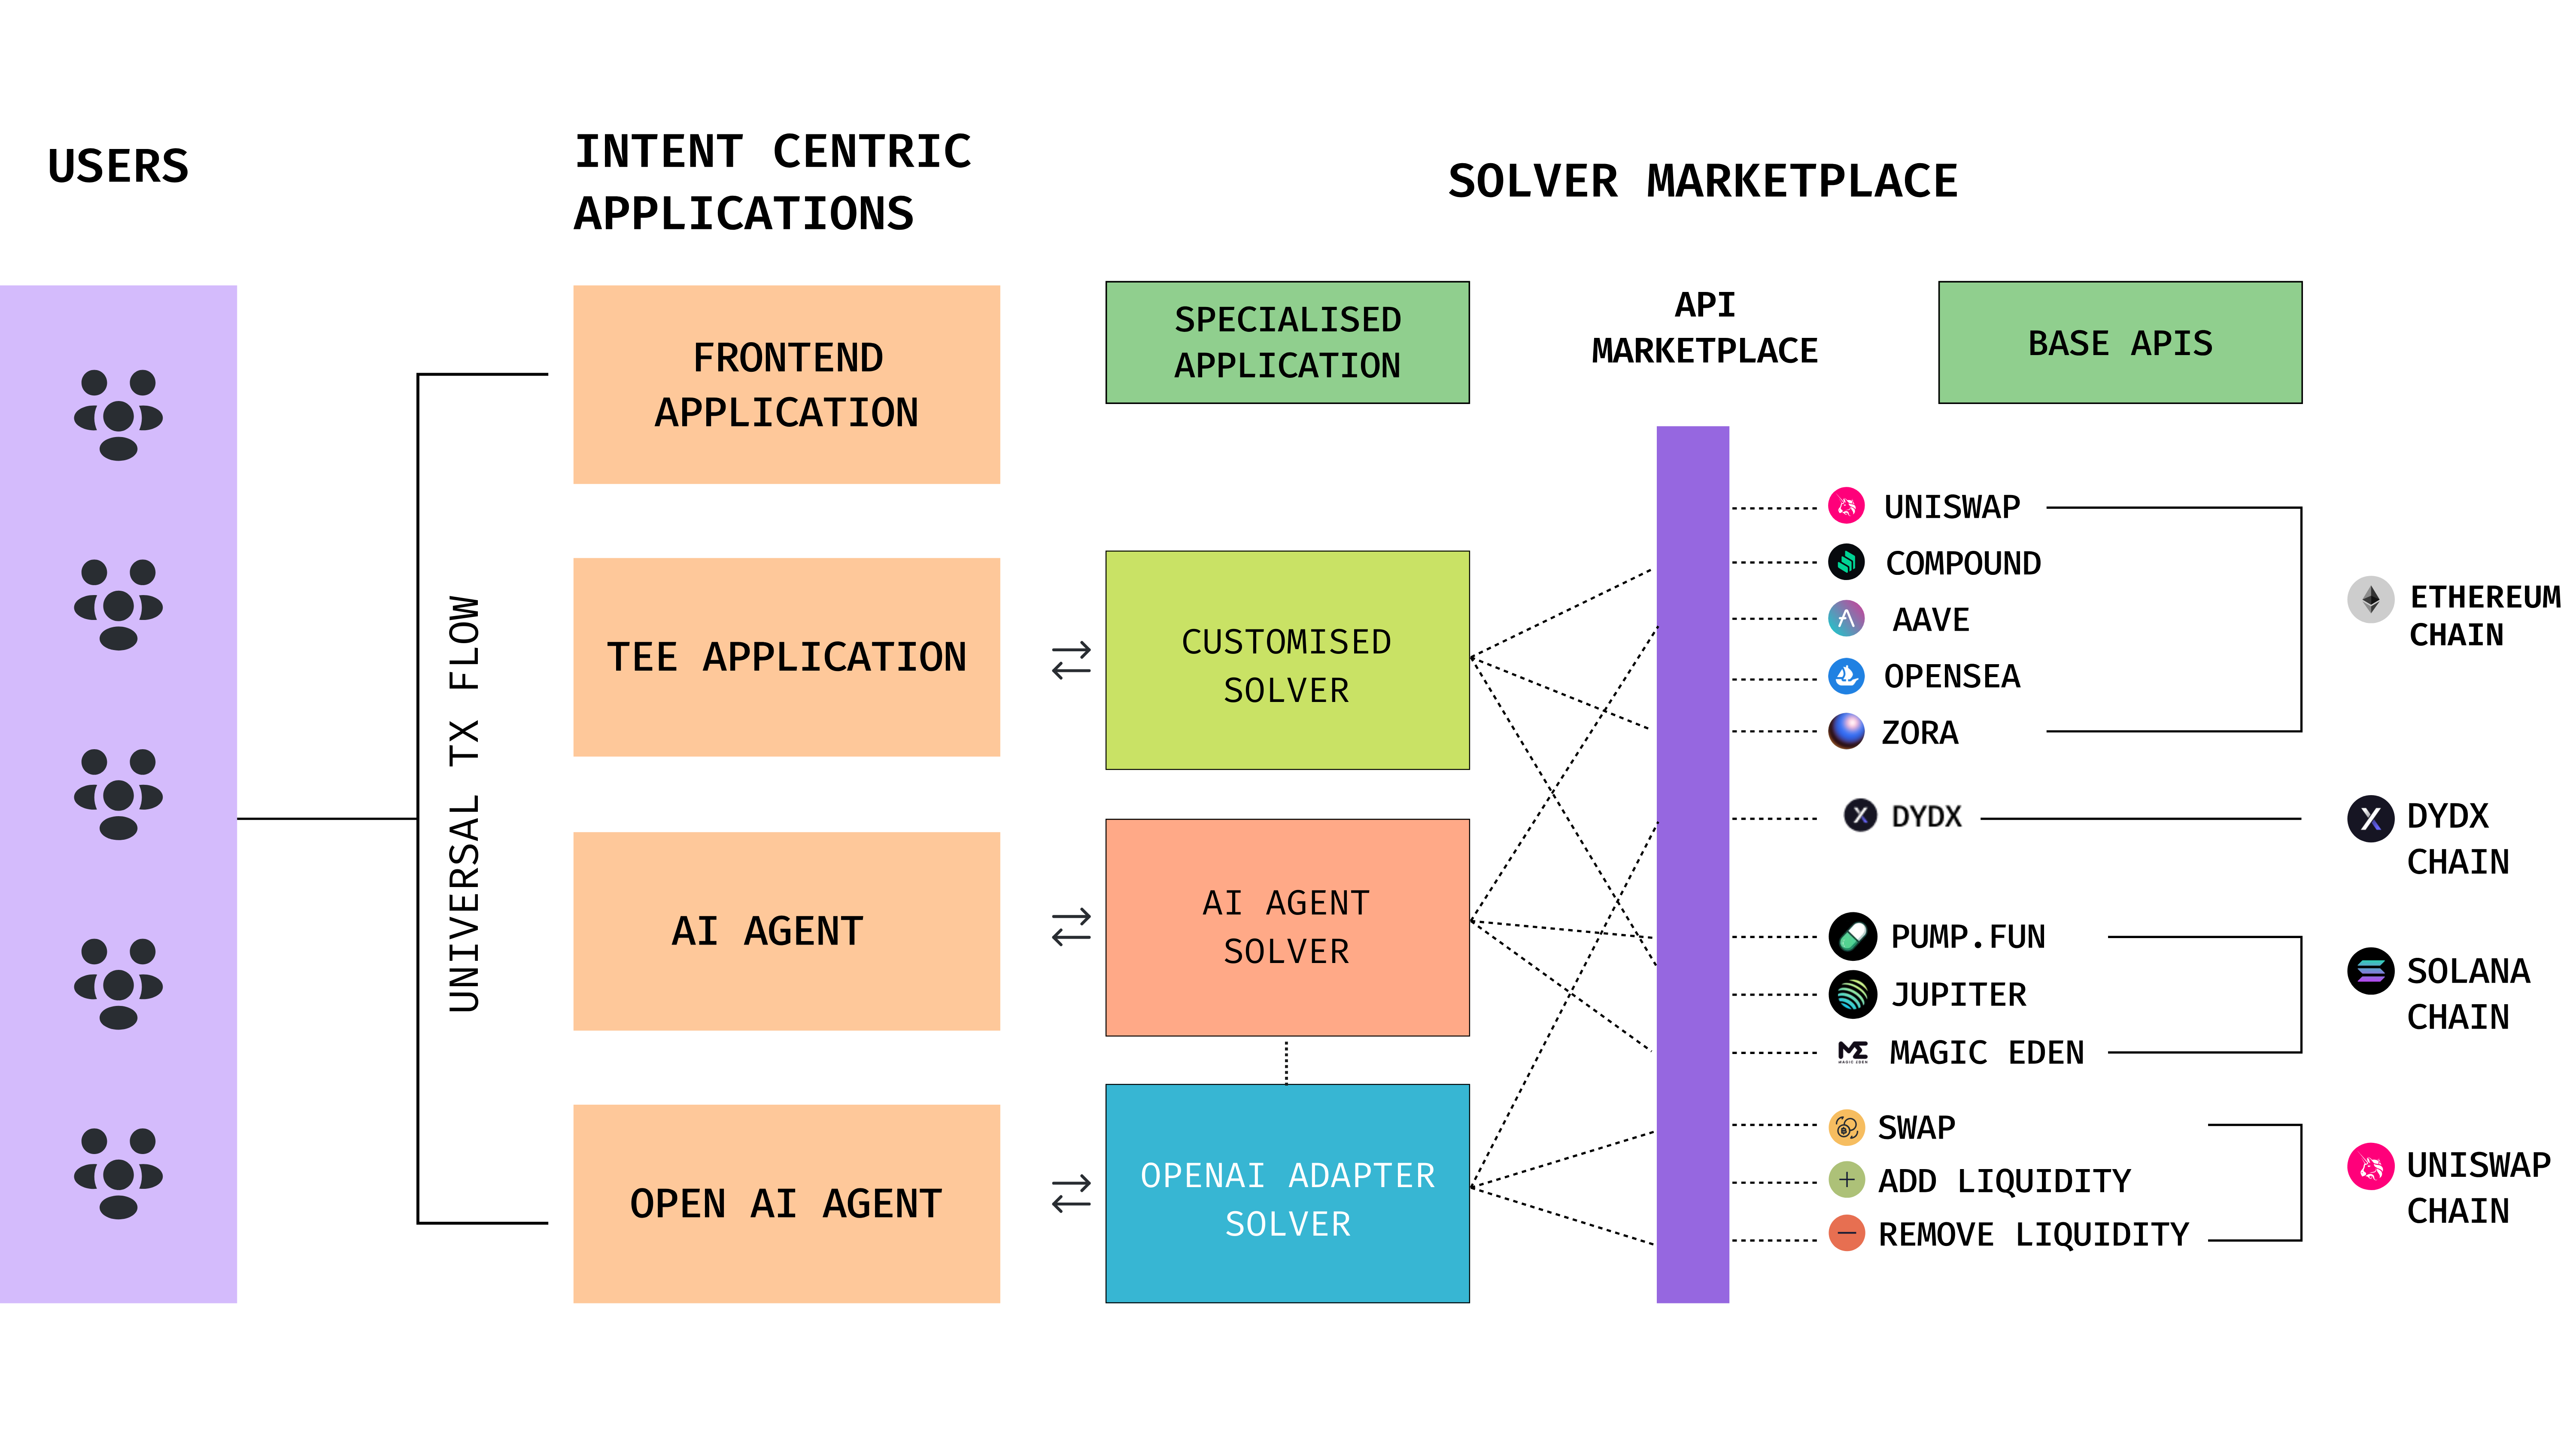
\includegraphics[width=0.9\linewidth]{figure/builder.png}
    \caption{Builder Marketplace Overview}
    \label{fig:builder}
\end{figure}

Beyond these dApp modules, developers can build customized solvers by merging functionalities from multiple modules. This allows for flexible and composable solutions, ensuring seamless cross-communication between solvers while optimizing execution paths. The Builder Marketplace supports universal transaction flows, catering to intent-centric applications, AI agents, and direct API calls from frontend applications. In addition, these specialized and base solvers feature dedicated interfaces, which can be used by intent-centric protocols and AI agents, further enhancing the interoperability, efficiency, and scalability of decentralized applications. By providing a structured yet adaptable framework, the Builder Marketplace serves as a powerful foundation for the next wave of blockchain-powered innovations.

By focusing on solver-driven execution, cross-chain interoperability, and a modular architecture, the Builder Marketplace empowers developers to create highly efficient and scalable solutions for decentralized applications. This ecosystem bridges the gap between disparate blockchain networks, offering a unified platform for seamless transaction execution and inter-chain communication.

\begin{figure}[h]
    \centering
    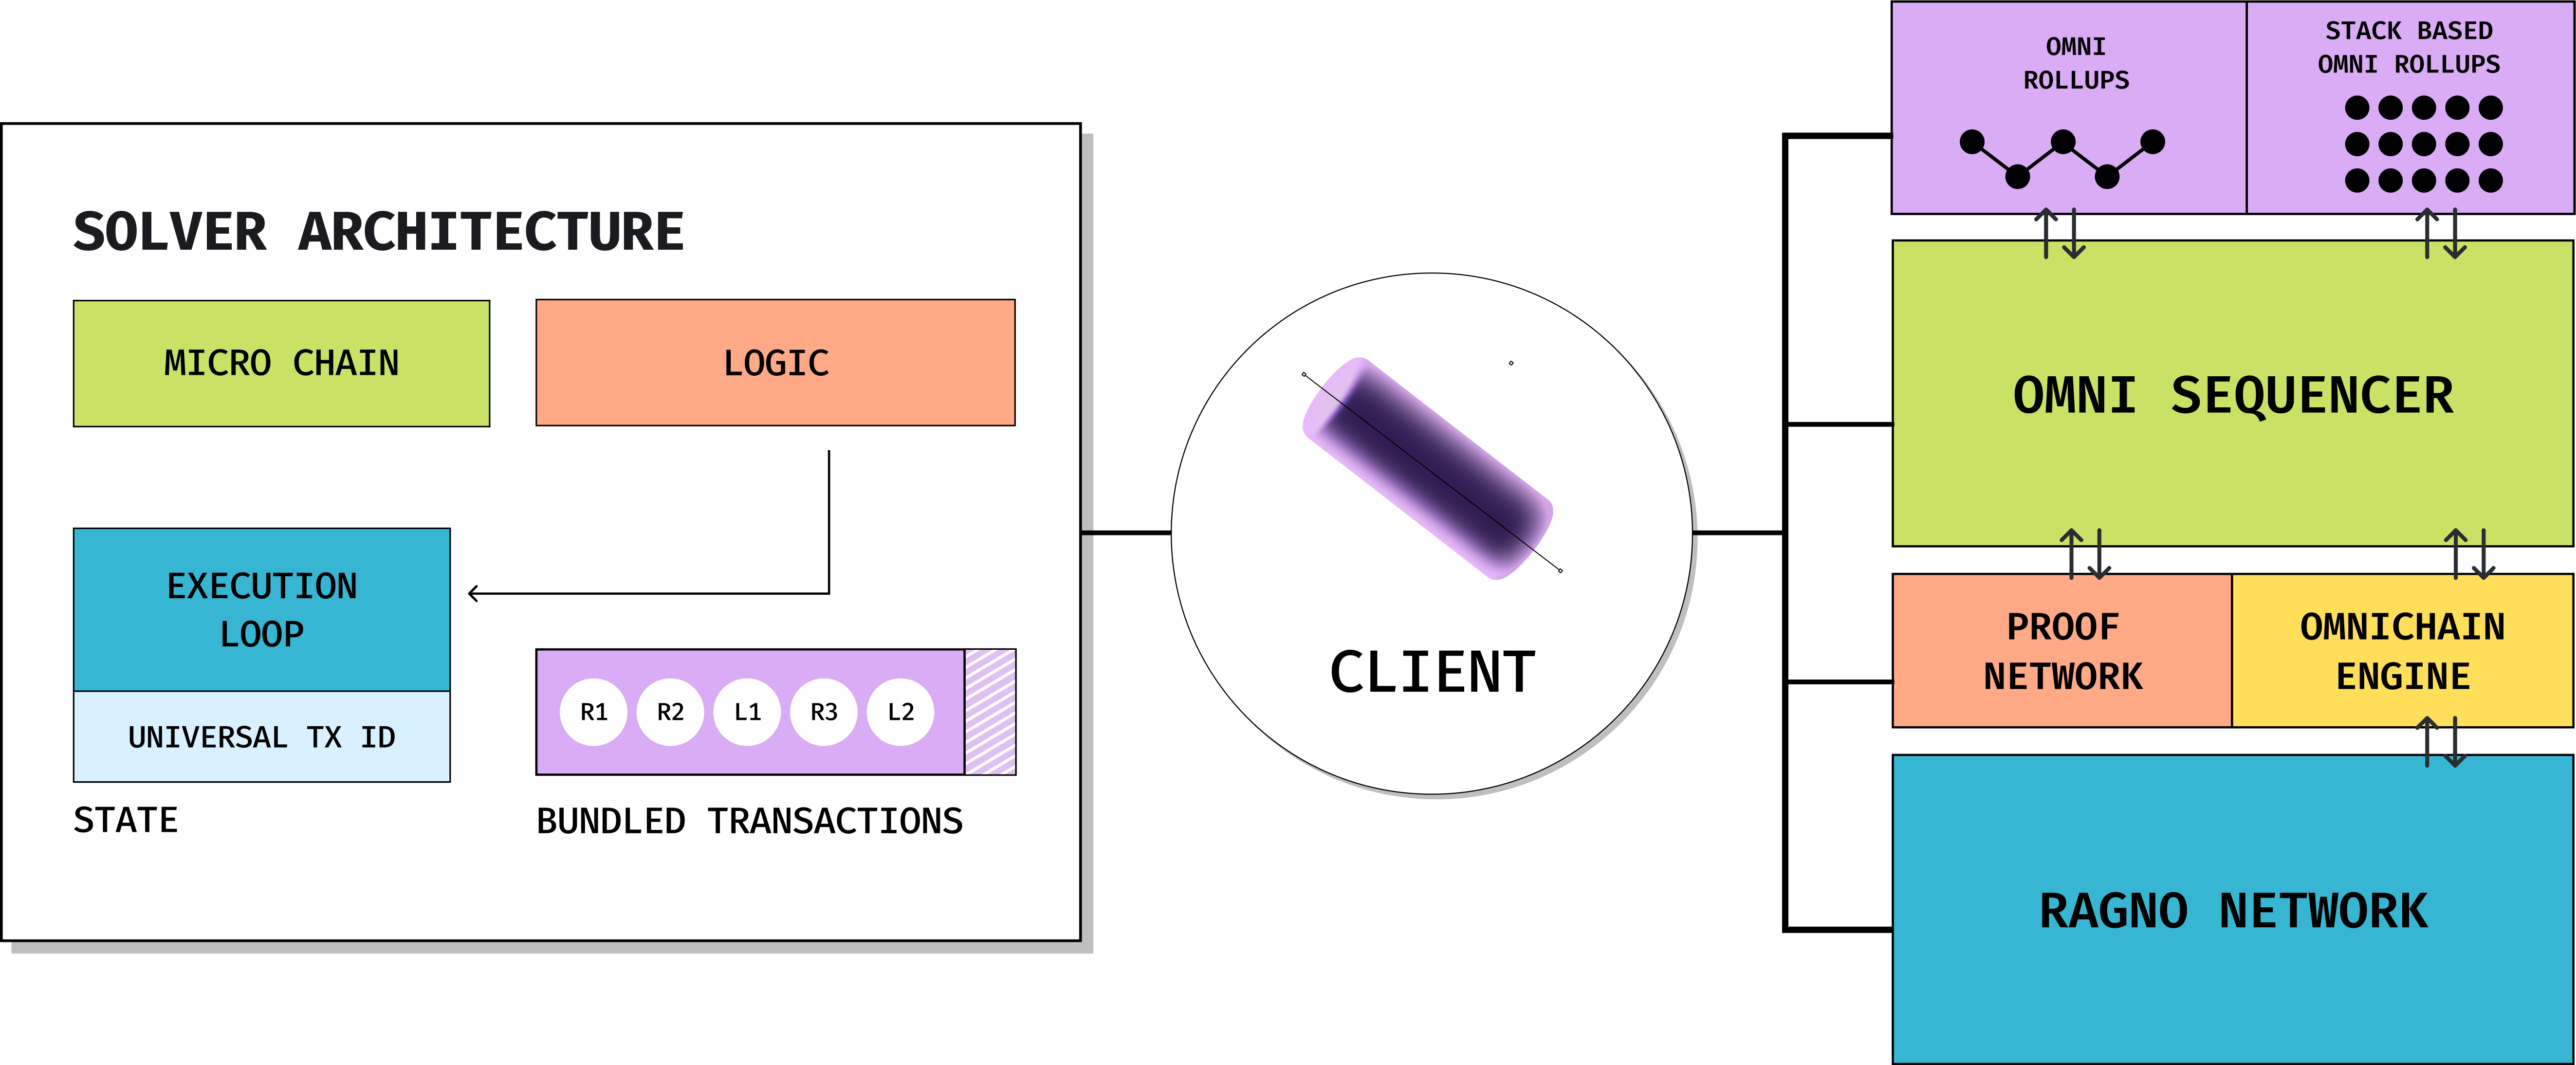
\includegraphics[width=0.9\linewidth]{figure/solver.png}
    \caption{Solver Illlustration}
    \label{fig:solver}
\end{figure}

\subsubsection{Solver Network}
The Solver Network operates as a decentralized network of solvers, each running its own Linera microchain~\cite{linera} to support various base API services. Each microchain contains critical components such as Rust-based logic for operations, addresses on different supported blockchain networks, and an information module for various base APIs. This modular architecture enables solvers to independently process transactions while maintaining interoperability within the broader solver ecosystem.

When a transaction is received, a solver performs rigorous verification processes. Validity checks ensure that input dependencies and execution feasibility are met, while authenticity is validated through user signatures. Once verified, the solver executes the transaction autonomously or collaborates with other solvers if additional resources or interactions are required to optimally fulfill the user intent.

Each solver is equipped with a dedicated client that facilitates integration with the Omni Sequencer, Prover Network, and Omnichain Engine. For omni-rollup transactions, the solver bundles transactions and forwards them to the Omni Sequencer, which orders them and dispatches them to the appropriate rollup for execution. The client continuously monitors these transactions, providing preconfirmation and confirmation updates to ensure reliable tracking and visibility of execution status.

For direct Layer 1 (L1) settlements using solver-owned addresses, solvers interact with Hermes validators for execution. To secure these transactions, the Threshold Signature Scheme (TSS) is used. Each solver’s client generates secret shares for its addresses on different blockchains, retaining one share while distributing the remaining shares among Hermes validators. This distribution is structured so that the solver's participation in the signing is essential to generate a valid transaction signature. Depending on the transaction type, the client interacts with the Omni Sequencer for rollup transactions or directly executes transactions on L1 chains via Hermes validator sets.

Direct settlement through solvers significantly enhances cross-chain transaction efficiency by reducing reliance on intermediary networks and ensuring streamlined execution. Using decentralized computation, advanced cryptographic mechanisms, and a modular execution environment, the Solver Network provides a robust foundation for executing user intents in a highly efficient and secure manner.

\subsubsection{Transaction Flow}
The transaction flow in the Builder Marketplace is designed to accommodate multiple types of transactions, ensuring seamless execution from the initiation to the final settlement. The different types of transaction include intent-centric transactions, AI-driven transactions, and direct API call transactions. Below is a breakdown of the transaction flow:
\begin{itemize}
    \item \textbf{Transaction Initiation}:

    Transactions can be initiated through intent-centric applications, AI agents, or direct API calls from front-end applications. Once a transaction request is submitted, the solver network analyzes it and determines the most efficient execution route.

    \item \textbf{Solver Selection and Processing}:

    The appropriate solver or group of solvers is chosen based on the characteristics of the transaction. They validate the transaction by verifying the input dependencies and feasibility. Cryptographic signatures are used to ensure authenticity.

    \item \textbf{Cross-Chain Communication and Execution}:

    For cross-chain transactions, solvers communicate via the microchain structure, utilizing integrated blockchain protocols for efficient execution. When omni-rollup handling is required, solvers bundle the transaction and forward it to the Omni Sequencer, which organizes and submits it to the appropriate rollup for execution.

    \item \textbf{Finalization and Settlement}:

    For omni-rollup transactions, the solver network monitors transaction progress, providing pre-confirmation and final confirmation updates. In the case of direct Layer 1 (L1) settlements, the solver collaborates with Hermes validators to execute the transaction. The final transaction state is then recorded on the relevant blockchain, ensuring both transparency and immutability.
    
    \item \textbf{Confirmation and Feedback}:
    
    Users receive updates on the transaction status in real time through the interface of the solver network. The system is designed to ensure efficient and secure transaction completion, optimizing minimal latency while maintaining maximum security.
\end{itemize}

    
This structured transaction flow ensures that the Builder Marketplace efficiently handles a diverse range of transactions while maintaining high performance, security, and scalability.

\section{Settlement Workflow}

In an omnichain ecosystem, transactions span across multiple blockchains, often requiring complex workflows to ensure correctness, security, and finality. Here is a breakdown of how the settlement process works, detailing the pre-confirmation, final confirmation, rollback mechanism, and error handling.

\textbf{Transaction Initiation}
\begin{itemize}
    \item Solver Network Transactions: Transactions initiated through solver networks involve multiple solvers that analyze the transaction request and select the most efficient path to execute it, often utilizing cross-chain bridges, microchains, or direct blockchain protocols.
    \item Omni-Rollup Transactions: For omni-rollup transactions, solvers bundle transactions, forward them to the Omni Sequencer, and submit them to the appropriate rollups for execution.
\end{itemize}


\textbf{Pre-Confirmation} 
\begin{itemize}
    \item Solver Network Transactions: The solver network begins by verifying inputs and ensuring that all dependencies are satisfied. For multi-chain transactions, solvers assess execution feasibility across involved blockchains, guaranteeing atomicity through commit/rollback mechanisms. During pre-confirmation, users receive real-time status updates, providing visibility into transaction progress and potential issues. Cryptographic signatures and proofs are validated to ensure authenticity and data integrity.
  
    \item Omni-Rollup Transactions: The Omni Sequencer processes the bundled transaction and begins the preconfirmation phase by verifying its feasibility within the rollup's context. It ensures that all participating rollups have adequate resources and that the transaction's data integrity remains intact. Once validated, a pre-confirmation status is sent to the user, indicating the transaction's readiness for final confirmation.
\end{itemize}



\textbf{Final Confirmation} 
\begin{itemize}
    \item Solver Network Transactions: After a successful preconfirmation, the solver network initiates transaction execution. For cross-chain transactions, solvers coordinate inter-chain dependencies and trigger the necessary operations, such as fund transfers or contract executions. Upon successful execution, the solvers update the final status of the transaction, confirming its completion, and submitting it to the appropriate blockchain or microchain. The final transaction state is then recorded on the respective blockchain, ensuring transparency and immutability.
    
    \item Omni-Rollup Transactions: Upon receiving pre-confirmation from all involved rollups, the Omni Sequencer issues the final confirmation to proceed with execution. It then submits the transaction to the respective rollup chains, where execution takes place. Once the transaction is successfully processed within each rollup, the final state is committed and synchronized across all rollups. Users receive final confirmation updates, ensuring transparency and verifying the successful completion of the omni-rollup transaction.
\end{itemize}


\textbf{Rollback Mechanism}

Rollback mechanisms are essential for ensuring that a transaction does not leave the system in an inconsistent or partially completed state in the event of failure. Rollback can happen after preconfirmation and before final settlement, but cannot happen after final settlement. 

The principle of atomicity ensures that all actions involved in the transaction are executed as a single, indivisible operation. If any part of the transaction fails, the entire transaction is rolled back.

\textbf{Two-Phase Commitment Protocol (2PC)~\cite{2pc}}:

\begin{itemize}
    \item Phase 1 - Locking Resources: In this phase, each participant in the transaction locks the assets they are going to send. These locks are usually time-bound, and the resources are held until the transaction is successfully committed or rolled back.
    \item Phase 2 - Finalizing or Rolling Back: Once all parties have confirmed that they are ready, the transaction is finalized. If any party fails to confirm or encounters an issue, the transaction is rolled back, and the locked assets are released or returned.
\end{itemize}
    
\begin{itemize}
    \item Solver Network Transactions: For each atomic transaction, a solver client verifies the successful locking of assets from all participating rollups. If asset locking on all participating rollups is successful within the specified time frame, the client commits to final execution and notifies all participating rollups accordingly. However, if the client fails to confirm successful asset locking on either rollup, it triggers a rollback, ensuring that all locked assets are released, thereby maintaining transaction atomicity.

    \item Omni-Rollup Transactions: For omni-rollup transactions, the rollback mechanism is managed by the rollup client. The source rollup client monitors the successful locking of assets across all participating rollups. If asset locking is confirmed on all rollups within the specified time frame, the client commits to final execution and notifies all participating rollups accordingly. However, if the client fails to confirm successful asset locking on any rollup, it triggers a rollback, ensuring that all locked assets are released, thereby preserving transaction atomicity.
\end{itemize}


\textbf{Error Handling}

Effective error handling ensures that any issues encountered during the transaction lifecycle are swiftly detected and managed.
\begin{itemize}
    \item Solver Network Transactions: During pre-confirmation, if input dependencies or feasibility checks fail, the solver network raises an error and notifies users with a detailed message explaining the cause. If an error occurs during execution (e.g., insufficient balance, contract failure), the transaction is halted, and the solver network initiates a rollback to maintain consistency. All errors are logged, and users receive real-time feedback. In cases of temporary failures, such as network congestion or brief outages, the system automatically retries the transaction to ensure successful completion.

    \item Omni-Rollup Transactions: If an omni-rollup transaction fails after pre-confirmation but before execution, the system automatically initiates a rollback across all affected rollups to maintain consistency. In the event of an execution failure, the Omni Sequencer handles the error by issuing a "transaction failed" status. Depending on the nature of the error, the transaction may be re-tried automatically, or users may be prompted to re-submit it. If rollback is not feasible due to an irrecoverable issue (e.g., a protocol bug or chain divergence), the system generates a detailed error message and suggests potential recovery options, such as modifying parameters for re-submission.
\end{itemize}


In an omnichain web ecosystem, the settlement workflow is complex, involving multiple stages to ensure transaction correctness. Pre-confirmation ensures eligibility, while final confirmation guarantees execution. Rollback mechanisms and error handling ensure that any failures are managed gracefully, preserving the integrity of the entire system. This process ensures that transactions are efficient, secure, and verifiable across multiple chains.

 


\section{Security}

The Omnichain Web introduces a paradigm shift in blockchain interoperability, enabling seamless asset and data transfer across multiple chains. However, this advancement comes with significant security challenges that require robust mechanisms to prevent exploits, bridge vulnerabilities, and unauthorized access. This section provides a comprehensive security overview that covers various security aspects.

\begin{itemize}
    \item[1.] Consensus Mechanisms: Proof-of-Stake (PoS) improves the security of interconnected chains by leveraging decentralized consensus models. It minimizes dependence on centralized validators and third-party intermediaries, ensuring that cross-chain transactions reach finality while preventing double-spending and rollback attacks.
    
    \item[2.] Cross-Chain Bridge Security: Enhance bridge security by implementing advanced cryptographic techniques like zero-knowledge proofs (ZKPs) and multiparty computation (MPC). Mitigating risks from blockchain reorganizations through optimistic and fraud-proof mechanisms. Automatically pausing transactions when detecting abnormal activity or potential attacks.

    \item[3.] Smart Contract Security: Using mathematical proofs to ensure the correctness of smart contracts. Conducting continuous security audits and incentivized vulnerability discovery programs. Implement safeguards to prevent recursive exploits in contract calls.

    \item[4.] Interoperability Layer Security: Prevent data tampering and oracle manipulation through cryptographic attestation. Ensuring secure state transitions across chains with cryptographic proofs such as zk-SNARKs and zk-STARKs. Using signed messages to block unauthorized state modifications.
\end{itemize}



\subsection{Dynamic TSS for Private OmniRollups and Solvers}
Dynamic Threshold Signature Schemes (TSS) play a critical role in improving security and efficiency in private roll-ups and solver networks. 
\begin{itemize}
    \item[1.] Decentralized Key Management: Eliminates single point of failure by distributing signing authority between multiple participants. Maintains liveness and robustness, ensuring operation even if some participants go offline or are compromised.

    \item[2.] Enhanced Privacy in Private Rollups: Private rollups prioritize confidentiality, with Threshold Signature Schemes (TSS) that securely distribute transaction signatures among designated parties without exposing private transaction details. This minimizes the risk of key leakage and unauthorized access.
    
    \item[3.] Resilience Against Attacks: Adaptive TSS dynamically reconfigures key shares to mitigate security breaches, ensuring resilience against Byzantine actors seeking to disrupt roll-up transactions.

    \item[4.] Secure Solver Network Participation: Solvers in DeFi protocols require a secure signing mechanism to submit solutions and interact with private order flows. TSS enables trust-minimized participation, safeguarding against collusion and unauthorized access.

    \item[5.] Efficient MultiChain Execution: Dynamic TSS enables multiple chains to coordinate execution securely without exposing sensitive data, strengthening cross-chain security while preserving scalability and performance.
\end{itemize}
The security of the omnichain web requires a multifaceted approach, integrating cryptographic proofs, decentralized validation, and threshold cryptography. Prover Network provides a robust security model for cross-chain transactions, ensuring trust-minimized execution. Additionally, dynamic TSS significantly enhances the security of private rollups and solver networks, offering strong protection against attacks while preserving privacy. As the omnichain ecosystem evolves, continuous security enhancements will be crucial to maintaining trust and interoperability across blockchain networks.
 
\section{Implementation}

To ensure the robustness and scalability of our omnichain architecture, we have set up a comprehensive testing environment using Docker, which incorporates key modules for the system’s components. These modules include Universal Layer 1, Hermes, Crawler, Narada, Operator, and the Operator Gateway Server. Each of these modules plays a critical role in the operation and validation of cross-chain transactions within the omnichain environment.

\begin{itemize}
    \item Universal Layer 1: Serving as the L1 for shared omni roll-ups, Universal Layer 1 is an EVM-compatible chain utilizing the DOJ native token and Dojima-specific contracts. It provides a secure and decentralized base layer for shared roll-ups, ensuring that cross-chain transactions can be validated and processed effectively.
  
    \item Hermes: A Cosmos SDK-based chain, Hermes functions as a bridge to connect Universal Layer 1 with other blockchain ecosystems. It is responsible for maintaining validators and liquidity between chains, acting as a critical connector for inter-chain transactions.

    \item Narada: This module maintains a suite of L1 clients, including Ethereum, Solana, Polkadot, and others, enabling Hermes to interact with a variety of blockchain networks. Narada currently supports GG20 TSS (Threshold Signature Scheme) and is in the process of integrating dynamic TSS based on the cggmp protocol, enhancing the security and flexibility of cross-chain interactions.

    \item Crawler: The Crawler module manages the list of registered operators and is responsible for establishing connections with different L1 chains via the Operator Gateway. It plays an essential role in the connectivity of the system.

    \item Operator: The Operator module runs nodes on various L1 chains and interfaces with the gateway server. It ensures that the interactions with different blockchains are seamless and secure, processing transactions and forwarding them as needed.

    \item Operator Gateway Server: The Gateway Server connects crawlers to operators, ensuring smooth data flow and operational integrity across different parts of the system.
\end{itemize}


For our testing purposes, we are utilizing Nitro-Espresso integration to test the Arbitrum Nitro roll-up with the Espresso sequencer, facilitating cross-chain transactions between Ethereum and omni version of Arbitrun Nitro rollup through our Universal L1. This provides us with a controlled environment to simulate real-world transactions and measure performance under various conditions.

The following system configurations are required to run the testing environment:

- Hermes: 8 GB RAM, 1 TB storage, 2 CPUs

- Narada: 2 CPUs, 2 GB RAM

- Crawler: 1 GB RAM, 1 CPU

- Universal Layer 1: 8 GB RAM, 2 CPUs, 1 TB storage

\textbf{Future Testing Plans}

We are in the process of scaling the system testing by dynamically adjusting the number of validators and processing a higher volume of input transactions. This will help ensure that the system can handle increased traffic and maintain its performance and security at larger scales. The goal is to continue refining the infrastructure and identify any potential bottlenecks that may arise in a production environment.

By continuously testing and improving the modules of the system and their interactions, our objective is to provide a robust, secure, and scalable omnichain architecture that meets the needs of decentralized applications and companies seeking to integrate Web3 technologies.


\section{Future Directions and Challenges}

\subsection{Future Direction}

The launch of WAAS (Web3 as a Service) marks a transformative leap in bridging the gap between Web2 and Web3 by enabling seamless integration through the Omnichain Web. As businesses, governments, and institutions seek to harness the power of decentralized technologies, WAAS provides a secure and scalable framework to connect their existing systems with the Web3 ecosystem. By leveraging the ZK Adapter and ZK Client, WAAS facilitates trustless interactions across multiple Layer 1 (L1) and Layer 2 (L2) blockchains, as well as rollups, ensuring interoperability without compromising security. This allows enterprises to efficiently manage critical operations such as deposits, withdrawals, contract interactions, and address management—all without relying on centralized intermediaries. With WAAS, Web2 entities can seamlessly onboard into Web3, unlocking new possibilities in a decentralized and interconnected digital landscape.

By offering omnichain capabilities, WAAS extends its reach beyond single-chain ecosystems, empowering Web2 entities, traditional institutions, governments, and banks to create their own decentralized operations. The ability to seamlessly connect with the entire Web3 space, while maintaining the security and trustlessness inherent in blockchain technology, is set to unlock new possibilities for innovation across industries. These advancements pave the way for a more inclusive and decentralized future, where organizations can access the power of blockchain without compromising security or scalability.

WAAS is poised to revolutionize the way companies engage with decentralized technologies, offering an efficient, transparent, and autonomous approach to cross-chain interactions. By enabling decentralized applications (dApps) and services to span across various blockchains, it fosters a new paradigm of collaboration and innovation, pushing the boundaries of what is possible in both Web2 and Web3 spaces. As a result, WAAS will play a key role in the ongoing development of decentralized finance (DeFi), supply chain management, identity systems, and beyond.

\subsubsection{Use Case: Existing L2's}
The ZK adapter plays a crucial role in transforming existing Layer 2 (L2) chains into fully omnichain ecosystems by enabling seamless cross-chain interoperability. Traditionally, L2 chains operate within isolated environments, limiting their ability to interact efficiently with other blockchains. By integrating the ZK Adapter, these chains gain the capability to verify and process cross-chain transactions in a secure, scalable, and trustless manner. The adapter leverages zero-knowledge proofs (ZKPs) to validate transactions across different blockchains without revealing sensitive information, ensuring both privacy and efficiency. Through this mechanism, all cross-chain transactions are routed through the Omnichain Web, a unified framework that standardizes communication between blockchains. This allows L2 networks to interact with multiple Layer 1 (L1) and L2 chains, as well as rollups, without requiring extensive protocol modifications or centralized intermediaries. As a result, L2 chains become inherently Omnichain, gaining access to a broader liquidity pool, improved composability, and greater adoption while maintaining their native security and scalability advantages.

\begin{figure}[h]
    \centering
    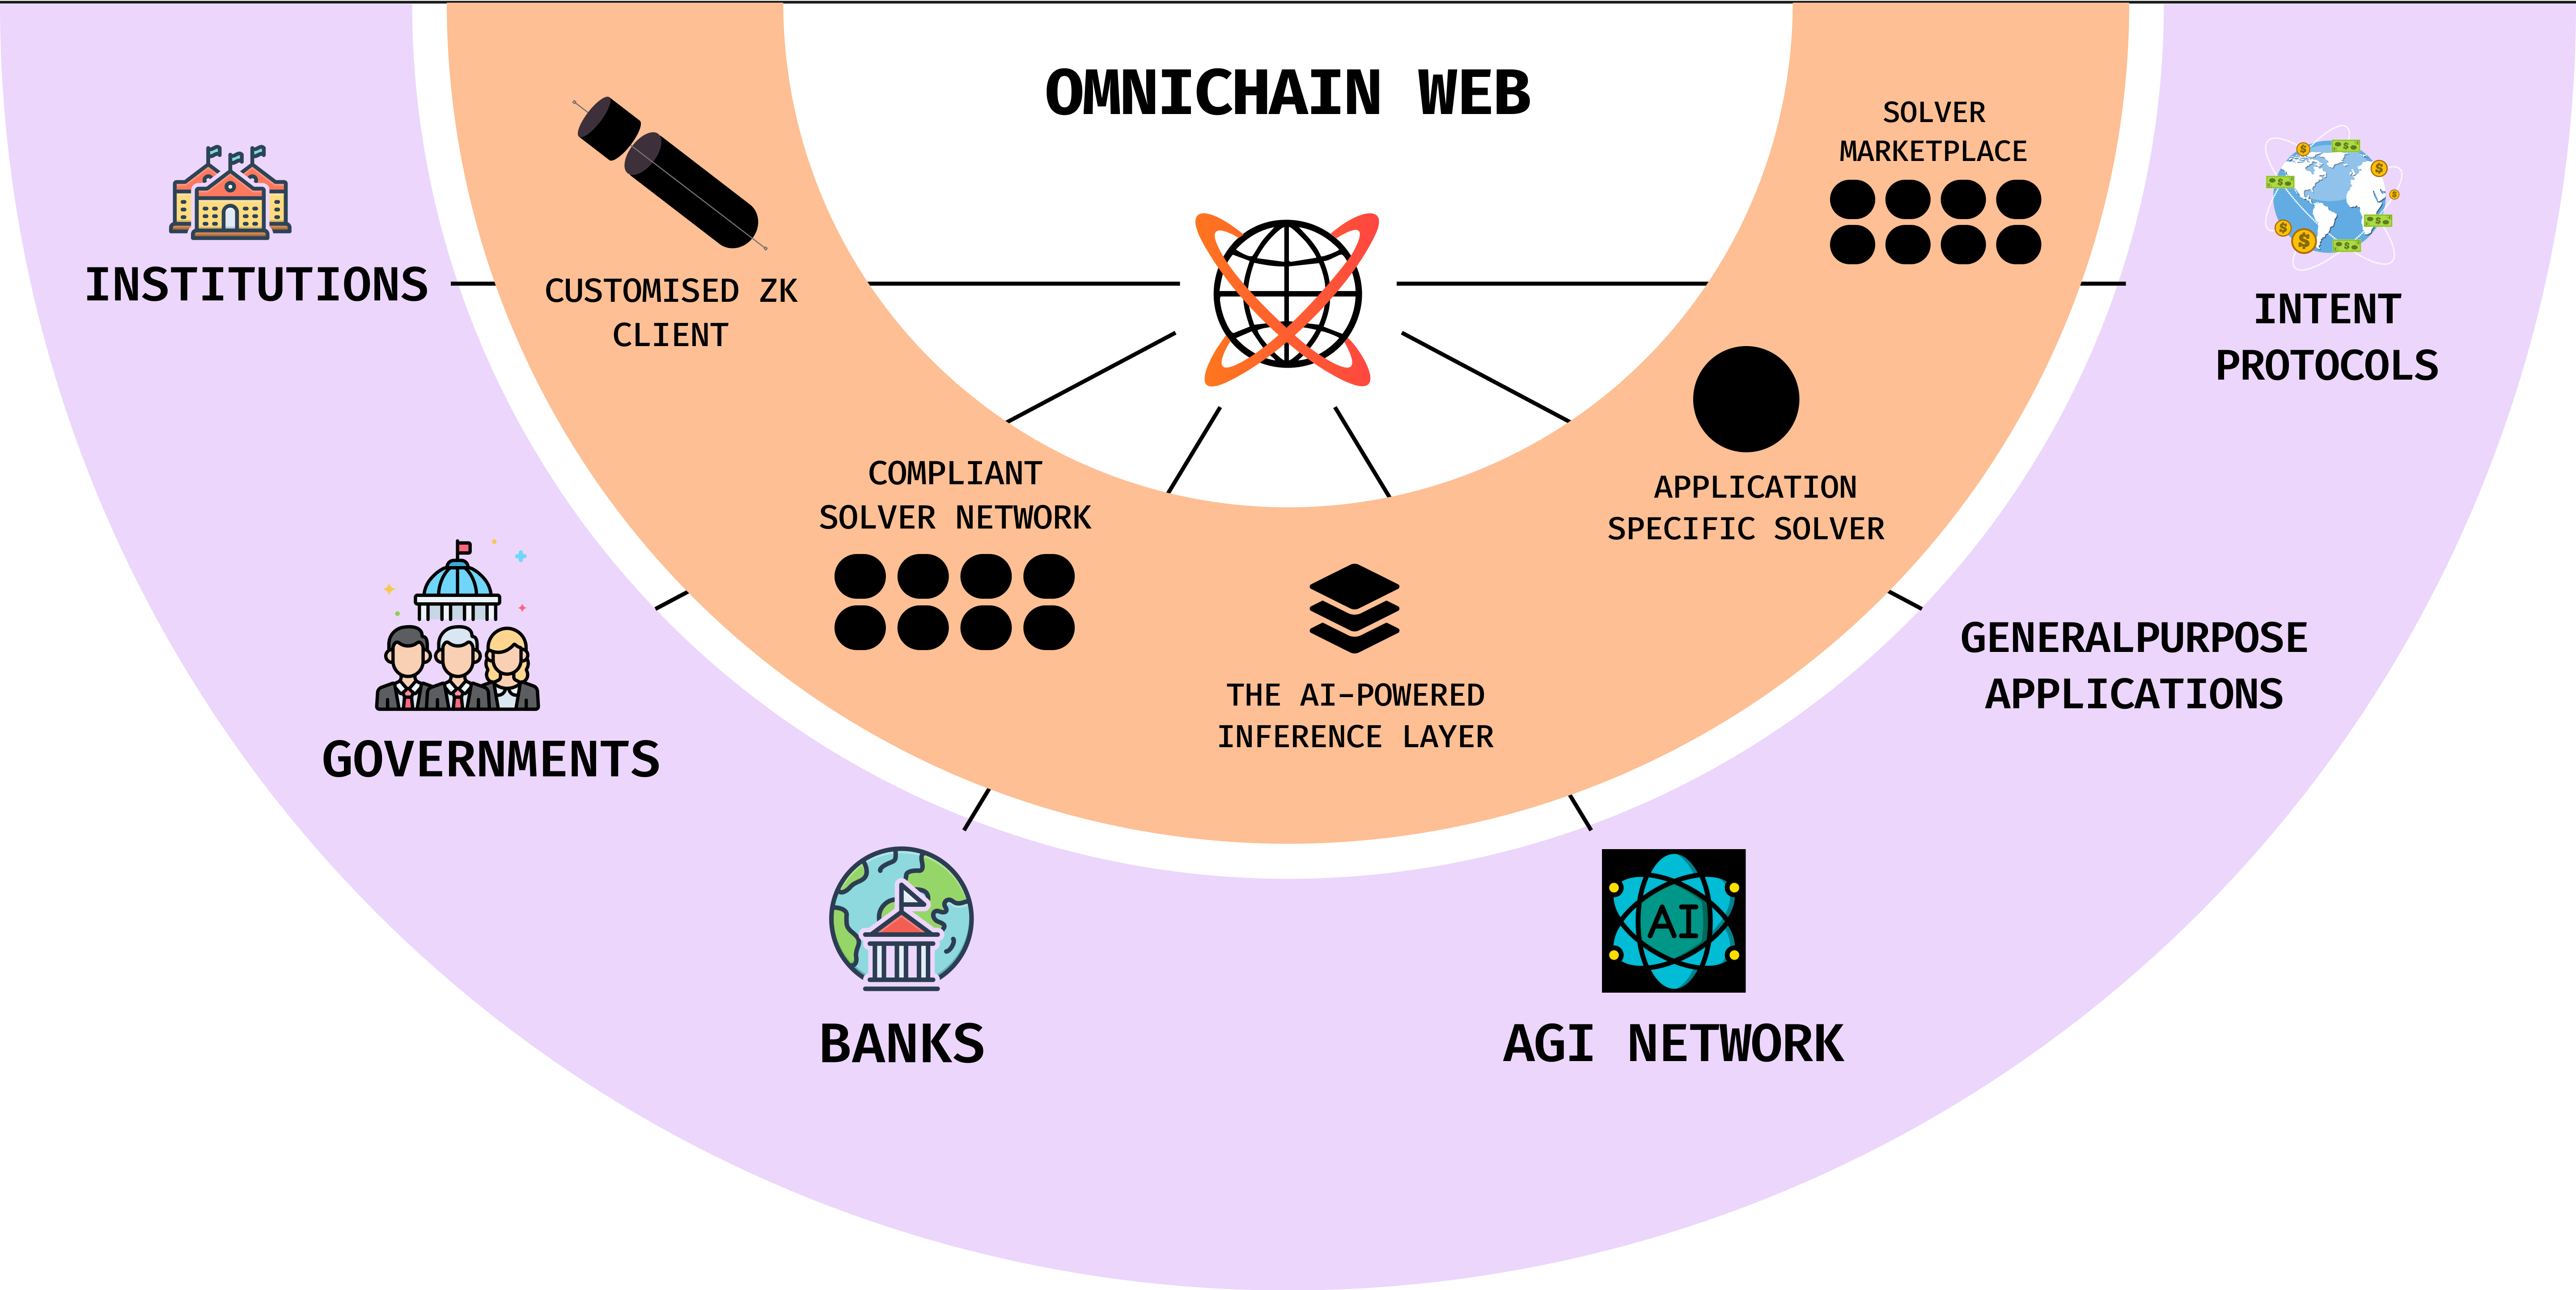
\includegraphics[width=0.9\linewidth]{figure/future.png}
    \caption{Mainstream Expansion}
    \label{fig:solver}
\end{figure}

\subsubsection{Use Cases: Bridging Web2 and Web3}

Currently, Web2 and traditional finance processes an astounding 6.7 billion transactions every day, but Web3 captures less than 1\% of this potential—a significant gap that highlights the scale of opportunity and the hurdles facing Web3 adoption. The next major opportunity lies in connecting Web2's vast scale with Web3's decentralized infrastructure. WAAS enables businesses and institutions to tap into the transformative power of blockchain technology without needing to overhaul their legacy systems. Following are some of the usecases.
 
\begin{itemize}
    \item Government and Public Sector Governments can use WAAS to integrate blockchain technology into public services such as voting, land registry, and identity management. With decentralized identity systems powered by Web3, governments can manage citizen data securely and privately without relying on centralized databases. Cross-chain interoperability ensures that these systems can interact with various blockchains to facilitate secure data transfer, ensuring broader adoption and improved efficiency. A government may also use WAAS to implement a decentralized voting system where voter identities are verified on a blockchain, ensuring transparency and security without relying on intermediaries.

    \item Financial Institutions and Banks Traditional banks are under increasing pressure to adapt to decentralized finance (DeFi). WAAS enables financial institutions to interact with multiple Layer 1 (L1) and Layer 2 (L2) blockchains, facilitating cross-chain transactions for activities such as cross-border payments, asset management, and decentralized lending platforms. By connecting Web2’s scale with Web3’s infrastructure, WAAS helps banks tap into the vast potential of Web3 without overhauling their existing systems. A bank using WAAS can offer customers seamless cross-border payments that utilize the most efficient blockchain, reducing fees and increasing transaction speed while maintaining compliance with regulatory standards.

    \item Institutions and Enterprises Enterprises looking to adopt blockchain for supply chain management, contract validation, or asset tracking can leverage WAAS to integrate Web3 solutions into their existing Web2 systems. WAAS ensures secure and scalable interactions between their traditional platforms and decentralized systems, offering the ability to track goods and services through immutable ledgers across multiple blockchains. A supply chain company could use WAAS to track products in real-time across multiple jurisdictions using blockchain, ensuring that all transactions (e.g., product movements, payments) are validated and traceable without the need for intermediaries.

    \item General-Purpose Applications Any general-purpose application, from social media platforms to gaming networks, can utilize WAAS to add decentralized features while maintaining their traditional user base. For instance, developers can create decentralized applications (dApps) that allow users to transfer assets, verify identities, or interact with smart contracts across multiple blockchains—all while ensuring the ease and familiarity of Web2 experiences. A gaming platform can leverage WAAS to integrate decentralized ownership of in-game assets, where players can buy, sell, and trade assets across various blockchain networks without losing the usability and performance of the platform.
\end{itemize}


By enabling cross-chain interactions, WAAS makes it possible for entities to securely and efficiently interact across various blockchain platforms, ensuring that they can participate in the Web3 ecosystem while benefiting from its scalability, security, and decentralization. As more industries explore the possibilities of Web3, WAAS will play a pivotal role in accelerating the adoption of blockchain technologies, helping to bridge the gap between today’s Web2-driven world and the decentralized future of Web3.

\subsection{Challenges}

Despite its immense potential, the deployment and adoption of WAAS face several significant challenges that need to be addressed as part of its continued evolution.

\begin{itemize}
    \item[1.] \textbf{Scalability and Performance in zk Systems}
    
   While the ZK adapter and the ZK client improve security, scalability remains a fundamental concern in the zk verification system.  Efficiently scaling WAAS to handle large-scale deployments while maintaining low latency and high throughput across different blockchains will require ongoing research and optimization of both the ZK protocols and the underlying infrastructure.

   \item[2.] \textbf{Regulatory and Legal Compliance}
   
   The decentralized and trustless nature of Web3 introduces complexities when it comes to regulatory compliance, especially for traditional institutions such as banks and governments. Navigating the rapidly changing landscape of blockchain regulation, including issues related to data privacy, anti-money laundering (AML), and know-your-customer (KYC) requirements, will be critical. WAAS must find ways to enable decentralized operations while complying with these regulations, ensuring that Web3 integrations do not conflict with existing legal frameworks.

    \item[3.] \textbf{Adoption and Education}
    
   One of the key challenges for WAAS will be adoption by Web2 companies and traditional institutions. Many of these organizations have limited experience with decentralized technologies and may be hesitant to adopt Web3 solutions due to perceived complexity or lack of understanding. WAAS will need to offer easy-to-use tools, comprehensive support, and educational resources to help these entities make the transition to decentralized operations smoothly. Convincing these organizations of the tangible benefits—such as cost savings, enhanced security, and greater efficiency—of integrating with Web3 will require a concerted effort in demonstrating value and fostering trust in the system.
\end{itemize}


\subsection{Conclusion}


The Omnichain Web is set to transform decentralized technology by addressing critical challenges in cross-chain interoperability, liquidity fragmentation, execution efficiency, and capital flow management. Through the integration of omnichain rollups, cross-chain intent standardization, and a decentralized solver network, this architecture eliminates inefficiencies, optimizes liquidity utilization, and provides a unified framework for seamless execution across multiple L1 and L2 ecosystems.  

One of the most pressing issues in Web3 has been fragmented liquidity and execution inefficiencies across chains. The Omnichain Web solves this by enabling peer-to-peer liquidity rebalancing, reducing reliance on centralized bridges that are often prone to security vulnerabilities. Additionally, the solver network, powered by omni-rollups, ensures efficient cross-chain intent fulfillment by netting complementary transactions, thereby minimizing capital inefficiencies and enhancing execution speed.  

Furthermore, the adoption of Dynamic Threshold Signature Scheme (TSS) enhances security by eliminating single points of failure in multi-party signing. Unlike static TSS, which requires pre-configured key shares, dynamic TSS allows flexible participation in signing operations, enabling more robust validator and solver rotation while maintaining decentralized security guarantees.  

The Ragno Network plays a pivotal role in enabling secure, scalable, and decentralized state management within the Omnichain Web. By ensuring deterministic state synchronization across omnichain rollups, Ragno provides a consistent execution environment where solvers can efficiently process intents, manage liquidity, and rebalance capital across various blockchains. This eliminates settlement risks and ensures trust-minimized execution, making cross-chain transactions more efficient and secure.  

  
Looking ahead, the Omnichain Web aims to enhance solver network capabilities by integrating AI-driven solvers for optimal liquidity management and efficient intent execution. Additionally, it seeks to develop regulatory-friendly solutions tailored for enterprises, institutions, and governments through its Web3-as-a-Service (WAAS) offerings. By eliminating inefficiencies in blockchain interoperability and enabling seamless cross-chain interactions, the Omnichain Web is positioned to become the foundation of the next-generation Web3 economy, effectively bridging the gap between Web2 and Web3 in a scalable and sustainable way. 
%----------------------------------------------------------------------------------------
% Bibliography
%----------------------------------------------------------------------------------------
\newpage % Includes a new page

\pagenumbering{roman} % Changes page numbering to roman page numbers
%\bibliography{literature}

\bibliography{literature.bib} % Add the filename of your bibliography
\bibliographystyle{plain} % Defines your bibliography style
%\begin{thebibliography}{9}
%\bibitem{www}
%Berners-Lee, T. Weaving the Web: The original design and ultimate destiny of %the World Wide Web by its inventor. Harper San Francisco, 1999.

%\end{thebibliography}

%\input{content/9B-declaration} 


%---------------------------------------------------------------------------------

\end{document}
